\documentclass[]{book}
\usepackage{lmodern}
\usepackage{amssymb,amsmath}
\usepackage{ifxetex,ifluatex}
\usepackage{fixltx2e} % provides \textsubscript
\ifnum 0\ifxetex 1\fi\ifluatex 1\fi=0 % if pdftex
  \usepackage[T1]{fontenc}
  \usepackage[utf8]{inputenc}
\else % if luatex or xelatex
  \ifxetex
    \usepackage{mathspec}
  \else
    \usepackage{fontspec}
  \fi
  \defaultfontfeatures{Ligatures=TeX,Scale=MatchLowercase}
\fi
% use upquote if available, for straight quotes in verbatim environments
\IfFileExists{upquote.sty}{\usepackage{upquote}}{}
% use microtype if available
\IfFileExists{microtype.sty}{%
\usepackage{microtype}
\UseMicrotypeSet[protrusion]{basicmath} % disable protrusion for tt fonts
}{}
\usepackage[margin=1in]{geometry}
\usepackage{hyperref}
\hypersetup{unicode=true,
            pdftitle={EPIB 607: Inferential Statistics},
            pdfauthor={Sahir Bhatnagar and James Hanley},
            pdfborder={0 0 0},
            breaklinks=true}
\urlstyle{same}  % don't use monospace font for urls
\usepackage{natbib}
\bibliographystyle{apalike}
\usepackage{color}
\usepackage{fancyvrb}
\newcommand{\VerbBar}{|}
\newcommand{\VERB}{\Verb[commandchars=\\\{\}]}
\DefineVerbatimEnvironment{Highlighting}{Verbatim}{commandchars=\\\{\}}
% Add ',fontsize=\small' for more characters per line
\usepackage{framed}
\definecolor{shadecolor}{RGB}{248,248,248}
\newenvironment{Shaded}{\begin{snugshade}}{\end{snugshade}}
\newcommand{\KeywordTok}[1]{\textcolor[rgb]{0.13,0.29,0.53}{\textbf{#1}}}
\newcommand{\DataTypeTok}[1]{\textcolor[rgb]{0.13,0.29,0.53}{#1}}
\newcommand{\DecValTok}[1]{\textcolor[rgb]{0.00,0.00,0.81}{#1}}
\newcommand{\BaseNTok}[1]{\textcolor[rgb]{0.00,0.00,0.81}{#1}}
\newcommand{\FloatTok}[1]{\textcolor[rgb]{0.00,0.00,0.81}{#1}}
\newcommand{\ConstantTok}[1]{\textcolor[rgb]{0.00,0.00,0.00}{#1}}
\newcommand{\CharTok}[1]{\textcolor[rgb]{0.31,0.60,0.02}{#1}}
\newcommand{\SpecialCharTok}[1]{\textcolor[rgb]{0.00,0.00,0.00}{#1}}
\newcommand{\StringTok}[1]{\textcolor[rgb]{0.31,0.60,0.02}{#1}}
\newcommand{\VerbatimStringTok}[1]{\textcolor[rgb]{0.31,0.60,0.02}{#1}}
\newcommand{\SpecialStringTok}[1]{\textcolor[rgb]{0.31,0.60,0.02}{#1}}
\newcommand{\ImportTok}[1]{#1}
\newcommand{\CommentTok}[1]{\textcolor[rgb]{0.56,0.35,0.01}{\textit{#1}}}
\newcommand{\DocumentationTok}[1]{\textcolor[rgb]{0.56,0.35,0.01}{\textbf{\textit{#1}}}}
\newcommand{\AnnotationTok}[1]{\textcolor[rgb]{0.56,0.35,0.01}{\textbf{\textit{#1}}}}
\newcommand{\CommentVarTok}[1]{\textcolor[rgb]{0.56,0.35,0.01}{\textbf{\textit{#1}}}}
\newcommand{\OtherTok}[1]{\textcolor[rgb]{0.56,0.35,0.01}{#1}}
\newcommand{\FunctionTok}[1]{\textcolor[rgb]{0.00,0.00,0.00}{#1}}
\newcommand{\VariableTok}[1]{\textcolor[rgb]{0.00,0.00,0.00}{#1}}
\newcommand{\ControlFlowTok}[1]{\textcolor[rgb]{0.13,0.29,0.53}{\textbf{#1}}}
\newcommand{\OperatorTok}[1]{\textcolor[rgb]{0.81,0.36,0.00}{\textbf{#1}}}
\newcommand{\BuiltInTok}[1]{#1}
\newcommand{\ExtensionTok}[1]{#1}
\newcommand{\PreprocessorTok}[1]{\textcolor[rgb]{0.56,0.35,0.01}{\textit{#1}}}
\newcommand{\AttributeTok}[1]{\textcolor[rgb]{0.77,0.63,0.00}{#1}}
\newcommand{\RegionMarkerTok}[1]{#1}
\newcommand{\InformationTok}[1]{\textcolor[rgb]{0.56,0.35,0.01}{\textbf{\textit{#1}}}}
\newcommand{\WarningTok}[1]{\textcolor[rgb]{0.56,0.35,0.01}{\textbf{\textit{#1}}}}
\newcommand{\AlertTok}[1]{\textcolor[rgb]{0.94,0.16,0.16}{#1}}
\newcommand{\ErrorTok}[1]{\textcolor[rgb]{0.64,0.00,0.00}{\textbf{#1}}}
\newcommand{\NormalTok}[1]{#1}
\usepackage{longtable,booktabs}
\usepackage{graphicx,grffile}
\makeatletter
\def\maxwidth{\ifdim\Gin@nat@width>\linewidth\linewidth\else\Gin@nat@width\fi}
\def\maxheight{\ifdim\Gin@nat@height>\textheight\textheight\else\Gin@nat@height\fi}
\makeatother
% Scale images if necessary, so that they will not overflow the page
% margins by default, and it is still possible to overwrite the defaults
% using explicit options in \includegraphics[width, height, ...]{}
\setkeys{Gin}{width=\maxwidth,height=\maxheight,keepaspectratio}
\IfFileExists{parskip.sty}{%
\usepackage{parskip}
}{% else
\setlength{\parindent}{0pt}
\setlength{\parskip}{6pt plus 2pt minus 1pt}
}
\setlength{\emergencystretch}{3em}  % prevent overfull lines
\providecommand{\tightlist}{%
  \setlength{\itemsep}{0pt}\setlength{\parskip}{0pt}}
\setcounter{secnumdepth}{5}
% Redefines (sub)paragraphs to behave more like sections
\ifx\paragraph\undefined\else
\let\oldparagraph\paragraph
\renewcommand{\paragraph}[1]{\oldparagraph{#1}\mbox{}}
\fi
\ifx\subparagraph\undefined\else
\let\oldsubparagraph\subparagraph
\renewcommand{\subparagraph}[1]{\oldsubparagraph{#1}\mbox{}}
\fi

%%% Use protect on footnotes to avoid problems with footnotes in titles
\let\rmarkdownfootnote\footnote%
\def\footnote{\protect\rmarkdownfootnote}

%%% Change title format to be more compact
\usepackage{titling}

% Create subtitle command for use in maketitle
\newcommand{\subtitle}[1]{
  \posttitle{
    \begin{center}\large#1\end{center}
    }
}

\setlength{\droptitle}{-2em}

  \title{EPIB 607: Inferential Statistics}
    \pretitle{\vspace{\droptitle}\centering\huge}
  \posttitle{\par}
    \author{Sahir Bhatnagar and James Hanley}
    \preauthor{\centering\large\emph}
  \postauthor{\par}
      \predate{\centering\large\emph}
  \postdate{\par}
    \date{2018-10-06}

\usepackage{booktabs}
\usepackage{longtable}
\usepackage[bf,singlelinecheck=off]{caption}

\let\originaltabular\tabular
\let\endoriginaltabular\endtabular
\renewenvironment{tabular}[1]{%
  \begingroup%
  \centering%
  \originaltabular{#1}}%
  {\endoriginaltabular\endgroup}

\usepackage{ifxetex,ifluatex}
\usepackage{fixltx2e} % provides \textsubscript
\ifnum 0\ifxetex 1\fi\ifluatex 1\fi=0 % if pdftex
  \usepackage[$if(fontenc)$$fontenc$$else$T1$endif$]{fontenc}
  \usepackage[utf8]{inputenc}
\else % if luatex or xelatex
  \makeatletter
  \@ifpackageloaded{fontspec}{}{\usepackage{fontspec}}
  \makeatother
  \defaultfontfeatures{Ligatures=TeX,Scale=MatchLowercase}
  \makeatletter
  \@ifpackageloaded{soul}{
     \renewcommand\allcapsspacing[1]{{\addfontfeature{LetterSpace=15}#1}}
     \renewcommand\smallcapsspacing[1]{{\addfontfeature{LetterSpace=10}#1}}
   }{}
  \makeatother
\fi

\usepackage{graphicx}
\setkeys{Gin}{width=\linewidth,totalheight=\textheight,keepaspectratio}

\usepackage{units}

% multiplecol
\usepackage{multicol}

% strikeout
\usepackage[normalem]{ulem}

% morefloats
\usepackage{morefloats}

% tightlist macro required by pandoc >= 1.14
\providecommand{\tightlist}{%
  \setlength{\itemsep}{0pt}\setlength{\parskip}{0pt}}



%% -- tint overrides
%% fonts, using roboto (condensed) as default
\usepackage[sfdefault,condensed]{roboto}
%% also nice: \usepackage[default]{lato}

%% colored links, setting 'borrowed' from RJournal.sty with 'Thanks, Achim!'
\RequirePackage{color}
\definecolor{link}{rgb}{0.1,0.1,0.8} %% blue with some grey
\hypersetup{
  colorlinks,%
  citecolor=link,%
  filecolor=link,%
  linkcolor=link,%
  urlcolor=link
}


%\usepackage{fontspec}
%\setmainfont[UprightFeatures={SmallCapsFont=AlegreyaSC-Regular}]{Alegreya}

\usepackage{framed,color}
\definecolor{shadecolor}{RGB}{248,248,248}

\renewcommand{\textfraction}{0.05}
\renewcommand{\topfraction}{0.8}
\renewcommand{\bottomfraction}{0.8}
\renewcommand{\floatpagefraction}{0.75}

%\renewenvironment{quote}{\begin{VF}}{\end{VF}}
%\let\oldhref\href
%\renewcommand{\href}[2]{#2\footnote{\url{#1}}}

\ifxetex
  \usepackage{letltxmacro}
  \setlength{\XeTeXLinkMargin}{1pt}
  \LetLtxMacro\SavedIncludeGraphics\includegraphics
  \def\includegraphics#1#{% #1 catches optional stuff (star/opt. arg.)
    \IncludeGraphicsAux{#1}%
  }%
  \newcommand*{\IncludeGraphicsAux}[2]{%
    \XeTeXLinkBox{%
      \SavedIncludeGraphics#1{#2}%
    }%
  }%
\fi

\makeatletter
\newenvironment{kframe}{%
\medskip{}
\setlength{\fboxsep}{.8em}
 \def\at@end@of@kframe{}%
 \ifinner\ifhmode%
  \def\at@end@of@kframe{\end{minipage}}%
  \begin{minipage}{\columnwidth}%
 \fi\fi%
 \def\FrameCommand##1{\hskip\@totalleftmargin \hskip-\fboxsep
 \colorbox{shadecolor}{##1}\hskip-\fboxsep
     % There is no \\@totalrightmargin, so:
     \hskip-\linewidth \hskip-\@totalleftmargin \hskip\columnwidth}%
 \MakeFramed {\advance\hsize-\width
   \@totalleftmargin\z@ \linewidth\hsize
   \@setminipage}}%
 {\par\unskip\endMakeFramed%
 \at@end@of@kframe}
\makeatother

\renewenvironment{Shaded}{\begin{kframe}}{\end{kframe}}

\newenvironment{rmdblock}[1]
  {
  \begin{itemize}
  \renewcommand{\labelitemi}{
    \raisebox{-.7\height}[0pt][0pt]{
      {\setkeys{Gin}{width=3em,keepaspectratio}\includegraphics{images/#1}}
    }
  }
  \setlength{\fboxsep}{1em}
  \begin{kframe}
  \item
  }
  {
  \end{kframe}
  \end{itemize}
  }
\newenvironment{rmdnote}
  {\begin{rmdblock}{note}}
  {\end{rmdblock}}
\newenvironment{rmdcaution}
  {\begin{rmdblock}{caution}}
  {\end{rmdblock}}
\newenvironment{rmdimportant}
  {\begin{rmdblock}{important}}
  {\end{rmdblock}}
\newenvironment{rmdtip}
  {\begin{rmdblock}{tip}}
  {\end{rmdblock}}
\newenvironment{rmdwarning}
  {\begin{rmdblock}{warning}}
  {\end{rmdblock}}

\usepackage{makeidx}
\makeindex

\urlstyle{tt}

\usepackage{amsthm}
\makeatletter
\def\thm@space@setup{%
  \thm@preskip=8pt plus 2pt minus 4pt
  \thm@postskip=\thm@preskip
}
\makeatother




%\usepackage[pagebackref=false,bookmarks]{hyperref}
\hypersetup{
	unicode=false,          
	pdftoolbar=true,        
	pdfmenubar=true,        
	pdffitwindow=false,     % window fit to page when opened
	pdfstartview={FitH},    % fits the width of the page to the window
	pdftitle={EPIB 607 Notes},    % title
	pdfauthor={Sahir Rai Bhatnagar},     % author
	pdfsubject={Subject},   % subject of the document
	pdfcreator={Sahir Rai Bhatnagar},   % creator of the document
	pdfproducer={Sahir Rai Bhatnagar}, % producer of the document
	pdfkeywords={}, % list of keywords
	pdfnewwindow=true,      % links in new window
	colorlinks=true,       % false: boxed links; true: colored links
	linkcolor=red,          % color of internal links (change box color with linkbordercolor)
	citecolor=blue,        % color of links to bibliography
	filecolor=black,      % color of file links
	urlcolor=blue         % color of external links
}


%\frontmatter % turns off chapter numbering and uses roman numerals for page numbers;
% https://tex.stackexchange.com/questions/20538/what-is-the-right-order-when-using-frontmatter-tableofcontents-mainmatter
\usepackage{booktabs}
\usepackage{longtable}
\usepackage{array}
\usepackage{multirow}
\usepackage[table]{xcolor}
\usepackage{wrapfig}
\usepackage{float}
\usepackage{colortbl}
\usepackage{pdflscape}
\usepackage{tabu}
\usepackage{threeparttable}
\usepackage{threeparttablex}
\usepackage[normalem]{ulem}
\usepackage{makecell}

\usepackage{amsthm}
\newtheorem{theorem}{Theorem}[chapter]
\newtheorem{lemma}{Lemma}[chapter]
\theoremstyle{definition}
\newtheorem{definition}{Definition}[chapter]
\newtheorem{corollary}{Corollary}[chapter]
\newtheorem{proposition}{Proposition}[chapter]
\theoremstyle{definition}
\newtheorem{example}{Example}[chapter]
\theoremstyle{definition}
\newtheorem{exercise}{Exercise}[chapter]
\theoremstyle{remark}
\newtheorem*{remark}{Remark}
\newtheorem*{solution}{Solution}
\begin{document}
\maketitle

{
\setcounter{tocdepth}{1}
\tableofcontents
}
\part{Preface}\label{part-preface}

\chapter{Welcome}\label{welcome}

Welcome to the course notes for
\href{https://www.mcgill.ca/study/2018-2019/courses/epib-607}{EPIB 607:
Inferential Statistics} at McGill University.

\section{Objectives}\label{objectives}

The aim of this course is to provide students with basic principles of
statistical inference so that they can:

\begin{enumerate}
\def\labelenumi{\arabic{enumi}.}
\tightlist
\item
  Visualize/Analyze/Interpret data using statistical methods
  \textbf{with a computer}.
\item
  Understand the statistical results in a scientific paper.\\
\item
  Apply statistical methods in their own research.\\
\item
  Use the methods learned in this course as a foundation for more
  advanced biostatistics courses.
\end{enumerate}

\section{Audience}\label{audience}

The principal audience is researchers in the natural and social sciences
who haven't had an introductory course in statistics (or did have one a
long time ago). This audience accepts that statistics has penetrated the
life sciences pervasively and is required knowledge for both doing
research and understanding scientific papers.

\section{About these notes}\label{about-these-notes}

These notes are a collection of useful links, videos, online resources
and papers for an introductory course in statistics. The instructors
have found that no single book sufficiently teaches all the topics
covered in this course. Part of this is due to advancements in computing
which have far outpaced the publication of modern textbooks. Indeed, the
computer has replaced many of the calculations that were traditionally
taught to be done by hand. We direct the readers to what we think is a
good learning resource for a given topic (following the \textbf{Flipped
Classroom} strategy). We also provide our own commentary and notes when
we think its useful.

\section{R Code Conventions}\label{r-code-conventions}

We use \href{https://cran.r-project.org/}{\texttt{R}} code throughout
these notes. When \texttt{R} code is displayed\footnote{\url{https://raw.githubusercontent.com/coatless/spm/master/index.Rmd}}
it will be typeset using a \texttt{monospace} font with syntax
highlighting enabled to ensure the differentiation of functions,
variables, and so on. For example, the following adds 1 to 1

\begin{Shaded}
\begin{Highlighting}[]
\NormalTok{a =}\StringTok{ }\NormalTok{1L }\OperatorTok{+}\StringTok{ }\NormalTok{1L}
\NormalTok{a}
\end{Highlighting}
\end{Shaded}

Each code segment may contain actual output from \texttt{R}. Such output
will appear in grey font prefixed by \texttt{\#\textgreater{}}. For
example, the output of the above code segment would look like so:

\begin{verbatim}
[1] 2
\end{verbatim}

\section{Rendering Mathematical
Formulae}\label{rendering-mathematical-formulae}

Throughout these notes, there will be mathematical symbols used to
express the material. Depending on the version of the book, there are
two different rendering engines.

\begin{itemize}
\tightlist
\item
  For the online version, the text uses
  \href{https://www.mathjax.org/}{MathJax} to render mathematical
  notation for the web. In the event the formulae does not load for a
  specific chapter, first try to refresh the page. 9 times out of 10 the
  issue is related to the software library not loading quickly. You can
  also right-click to see the corresponding LaTeX code used to produce
  the equation.\\
\item
  For the pdf version, the text is built using the recommended AMS LaTeX
  symbolic packages. As a result, there should be no issue displaying
  equations. An example of a mathematical rendering capabilities would
  be given as:
\end{itemize}

\[ a^2 + b^2 = c^2 \]

\section{Development}\label{development}

This book is built with
\href{https://github.com/rstudio/bookdown}{\textbf{bookdown}} and is
open source and freely available. This approach encourages
contributions, ensures reproducibility and provides access to the
material worldwide. The online version of the book is hosted at
\href{https://sahirbhatnagar.com/EPIB607}{sahirbhatnagar.com/EPIB607}
and kept up-to-date thanks to
\href{https://travis-ci.org/sahirbhatnagar/EPIB607}{Travis}. The entire
source code is available at
\url{https://github.com/sahirbhatnagar/EPIB607}.

If you notice any errors, we would be grateful if you would let us know
by filing an issue
\href{https://github.com/sahirbhatnagar/EPIB607/issues}{here} or making
a pull request by clicking the edit button in the top-left corner of the
text:

\begin{figure}
\centering

\includegraphics{images/edit_button.png}
\caption{}
\end{figure}

The version of the book you are reading now was built on 2018-10-06 and
was built on
\href{https://travis-ci.org/sahirbhatnagar/MATH697}{Travis}.

\section{About the authors}\label{about-the-authors}

\begin{longtable}[]{@{}cc@{}}
\toprule
Sahir Bhatnagar & James Hanley\tabularnewline
\midrule
\endhead
&\tabularnewline
\bottomrule
\end{longtable}

\begin{itemize}
\tightlist
\item
  Sahir R. Bhatnagar: Assistant Professor of Biostatistics - McGill
  University, Montreal, Canada.

  \begin{itemize}
  \tightlist
  \item
    Website: \url{https://sahirbhatnagar.com/}\\
  \item
    Twitter: \href{https://twitter.com/syfi_24}{syfi\_24}\\
  \item
    GitHub: \url{https://github.com/sahirbhatnagar}\\
  \end{itemize}
\item
  James A. Hanley: Professor of Biostatistics - McGill University,
  Montreal, Canada.

  \begin{itemize}
  \tightlist
  \item
    Webpage: \url{http://www.medicine.mcgill.ca/epidemiology/hanley/}
  \end{itemize}
\end{itemize}

\section{License}\label{license}

This work is licensed under a Creative Commons Attribution 4.0
International License

\chapter{Course Information}\label{course-information}

\begin{itemize}
\tightlist
\item
  Instructor: \href{mailto:sahir.bhatnagar@mcgill.ca}{Sahir Bhatnagar}\\
\item
  Teaching Assistants:

  \begin{itemize}
  \tightlist
  \item
    \href{mailto:kody.crowell@mail.mcgill.ca}{Kody Crowell},
    \texttt{kody.crowell@mail.mcgill.ca}, Mondays 2-3pm (Ab - Gi)
  \item
    \href{mailto:dewdunee.marasinghe@mail.mcgill.ca}{Himasara
    Marasinghe}, \texttt{dewdunee.marasinghe@mail.mcgill.ca}, Thursdays
    1-2pm (Ha - Pa)
  \item
    \href{mailto:guanbo.wang@mail.mcgill.ca}{Guanbo Wang},
    \texttt{guanbo.wang@mail.mcgill.ca}, Wednesdays 11:30am-12:30pm (Pl
    - Za)
  \end{itemize}
\item
  Website: \url{http://sahirbhatnagar.com/EPIB607/}\\
\item
  Lectures: Monday 11:30am - 1:30pm, Thursday 8:30am - 10:30am\\
\item
  Location: McMed 1034\\
\item
  Office Hours: TBD\\
\item
  Prerequisite(s): Calculus and Algebra\\
\item
  Texts: \emph{The Practice of Statistics in the Life Sciences}, 3nd
  Edition by Baldi \& Moore.\\
\item
  Midterm: October 29, 2018
\item
  Final: December 4, 2018
\end{itemize}

\section{Teaching strategy}\label{teaching-strategy}

This course will follow the \textbf{Flipped Classroom} model. Here,
students are expected to have engaged with the material before coming to
class (based on very precise pre-class instructions). The students will
then be expected to answer a series of conceptual multiple choice
questions using the
\href{https://mydalite.org/en/live/signup/form/NTc4}{DALITE} online
platform \citep{bhatnagar2016dalite}.

This allows the instructor to delegate the delivery of basic content and
definitions to textbooks and videos, and enforces the idea that students
cannot be simply passive recipients of information. This approach then
allows the professor to focus valuable class time on nurturing efficient
discussions surrounding the ideas within the content, guiding
interactive exploration of typical misconceptions, and promoting
collaborative problem solving with peers.

\section{A focus on computation}\label{a-focus-on-computation}

Classic introductory statistics textbooks were written during a time
when computers were still in their infancy. As such, even the newer
editions heavily rely on \emph{by-hand} computations such as looking up
tables for tail probabilities. We take a modern approach and introduce
computational methods in statistics with the statistical software
program \texttt{R}.

\section{DataCamp}\label{datacamp}

This class is supported by \href{https://www.datacamp.com/}{DataCamp},
the most intuitive learning platform for data science. Learn R, Python
and SQL the way you learn best through a combination of short expert
videos and hands-on-the-keyboard exercises. Take over 100+ courses by
expert instructors on topics such as importing data, data visualization
or machine learning and learn faster through immediate and personalised
feedback on every exercise.

\begin{figure}
\centering

\includegraphics{images/datacamp.png}
\caption{}
\end{figure}

You will be asked to complete some of the courses in DataCamp for
background reading or for assignments. You can sign up for a free
account at
\href{https://www.datacamp.com/groups/shared_links/4c7d78a632b557dfdd6618b3e8fac09495571fec}{this
link}. Note: you are required to sign up with a \texttt{@mail.mcgill.ca}
or \texttt{@mcgill.ca} email address.

\section{Grade Distribution}\label{grade-distribution}

\begin{tabular}{ll}
\toprule
 & \\
\midrule
Assignments & 40\%\\
DALITE & 15\%\\
Midterm & 15\%\\
Project & 10\%\\
Final Exam & 20\%\\
\bottomrule
\end{tabular}

\chapter{Target Syllabus}\label{target-syllabus}

\begin{tabular}{ll}
\toprule
Abbreviation & Description\\
\midrule
JH & James Hanley notes\\
EM & Erica Moodie notes\\
OS & Olli Saarela notes\\
AAO & Against all odds video series\\
B\&M & The practice of statistics in the life sciences by Baldi and Moore, 3rd edition\\
\addlinespace
Freedman & Statistics by Freedman, Pisani, Purves, Adhikari, 2nd edition\\
dataviz & Fundamentals of Data Visualization by Claus O. Wilke\\
\bottomrule
\end{tabular}

\section{Descriptive Statistics}\label{descriptive-statistics}

\begin{tabular}{lllll}
\toprule
Topic & Video & Readings & Exercise & DALITE\\
\midrule
Histograms & [AAO unit 3](https://www.learner.org/courses/againstallodds/unitpages/unit03.html) & [AAO unit 3, pages 1-6](https://www.learner.org/courses/againstallodds/pdfs/AgainstAllOdds\_StudentGuide\_Unit03.pdf\#page=1) & [AAO unit 3, Wafer Thickness pages 15-17](https://www.learner.org/courses/againstallodds/pdfs/AgainstAllOdds\_StudentGuide\_Unit03.pdf\#page=15) & --\\
Density Plots & -- & [dataviz chapter 7](https://serialmentor.com/dataviz/histograms-density-plots.html) & -- & --\\
Measures of Center & [AAO unit 4](https://www.learner.org/courses/againstallodds/unitpages/unit04.html) & [AAO unit 4, pages 1-6](https://www.learner.org/courses/againstallodds/pdfs/AgainstAllOdds\_StudentGuide\_Unit04.pdf\#page=1) & [AAO unit 4, Mean, Median and Distribution Shape pages 13-14](https://www.learner.org/courses/againstallodds/pdfs/AgainstAllOdds\_StudentGuide\_Unit04.pdf\#page=13) & --\\
Boxplots & [AAO unit 5](https://www.learner.org/courses/againstallodds/unitpages/unit05.html) & [AAO unit 5, pages 1-5](https://www.learner.org/courses/againstallodds/pdfs/AgainstAllOdds\_StudentGuide\_Unit05.pdf\#page=1) & -- & --\\
Standard Deviation & [AAO unit 6](https://www.learner.org/courses/againstallodds/unitpages/unit06.html) & [AAO unit 6, pages 1-3](https://www.learner.org/courses/againstallodds/pdfs/AgainstAllOdds\_StudentGuide\_Unit06.pdf\#page=1) & [AAO unit 4, Visualizing Standard Deviation pages 10-13](https://www.learner.org/courses/againstallodds/pdfs/AgainstAllOdds\_StudentGuide\_Unit06.pdf\#page=10) & --\\
Data Visualization & [Hans Rosling BBC](https://www.youtube.com/watch?v=jbkSRLYSojo) & [JH notes on Descriptives](https://www.dropbox.com/s/lomkigwypksudcn/DescriptiveStatistics.pdf?dl=0) & -- & --\\
\bottomrule
\end{tabular}

\section{Sampling Distributions}\label{sampling-distributions}

\begin{tabular}{lllll}
\toprule
Topic & Video & Readings & Exercise & DALITE\\
\midrule
Parameters and Statistics & -- & [[JH section 1]](https://www.dropbox.com/s/kr293cablb11nrm/Ch13SamplingDistributionsJH2018.pdf?dl=0) [[B\&M page 314]](https://www.dropbox.com/s/8u0j9lupv5pxqpm/Ch13SamplingDistributions.pdf?dl=0) & -- & --\\
Sampling Distributions & [AAO unit 22](https://www.learner.org/courses/againstallodds/unitpages/unit22.html) & [[AAO unit 22, pages 1-10]](https://www.learner.org/courses/againstallodds/pdfs/AgainstAllOdds\_StudentGuide\_Unit22.pdf) [[JH sections 2-6]](https://www.dropbox.com/s/kr293cablb11nrm/Ch13SamplingDistributionsJH2018.pdf?dl=0) [[B\&M pages 315-320]](https://www.dropbox.com/s/8u0j9lupv5pxqpm/Ch13SamplingDistributions.pdf?dl=0) & -- & --\\
Central Limit Theorem & [AAO unit 22](https://www.learner.org/courses/againstallodds/unitpages/unit22.html) & [B\&M pages 321-324](https://www.dropbox.com/s/8u0j9lupv5pxqpm/Ch13SamplingDistributions.pdf?dl=0) & -- & --\\
The Bootstrap & -- & [[Computer-Intensive Methods in Statistics]](http://folk.uio.no/deilerts/phd/docs/Efron-scientificamerican0583-116.pdf) [[Bootstrap confidence intervals ]](http://mosaic-web.org/go/SM2-technique/confidence-intervals.html) & -- & --\\
\bottomrule
\end{tabular}

\section{Introduction to Inference}\label{introduction-to-inference}

\begin{tabular}{lllll}
\toprule
Topic & Video & Readings & Exercise & DALITE\\
\midrule
Confidence Intervals & [AAO unit 24](https://www.learner.org/courses/againstallodds/unitpages/unit24.html) & [[AAO unit 24, pages 1-6]](https://www.learner.org/courses/againstallodds/pdfs/AgainstAllOdds\_StudentGuide\_Unit24.pdf) [[JH notes]](https://www.dropbox.com/s/epgqkz3g0qklcp9/Ch14ConfidenceIntervalsJH2018.pdf?dl=0) [[Standard deviation, standard error. Which 'standard' should we use?]](http://www.medicine.mcgill.ca/epidemiology/hanley/BionanoWorkshop/SD-SE.pdf) & -- & --\\
Tests of Significance and P-values & [AAO unit 25](https://www.learner.org/courses/againstallodds/unitpages/unit25.html) & [[AAO unit 25, pages 1-12]](https://www.learner.org/courses/againstallodds/pdfs/AgainstAllOdds\_StudentGuide\_Unit25.pdf) [[JH, What the p-value is not]](http://www.medicine.mcgill.ca/epidemiology/hanley/BionanoWorkshop/P-Values.pdf) & -- & --\\
\bottomrule
\end{tabular}

\section{One-sample Inference}\label{one-sample-inference}

\begin{tabular}{lllll}
\toprule
Topic & Video & Readings & Exercise & DALITE\\
\midrule
Means & [AAO unit 26](https://www.learner.org/courses/againstallodds/unitpages/unit26.html) & [[AAO unit 26, pages 1-11]](https://www.learner.org/courses/againstallodds/pdfs/AgainstAllOdds\_StudentGuide\_Unit26.pdf) [[B\&M chapter 11]](https://www.dropbox.com/s/hihe04t0v5e8evi/Ch11TheNormalDistributions.pdf?dl=0) [[B\&M chapter 17]](https://www.dropbox.com/s/qs58c54zh1kui4d/Ch17InferenceAboutPopulationMean.pdf?dl=0) & -- & --\\
Proportions & [AAO unit 28](https://www.learner.org/courses/againstallodds/unitpages/unit28.html) & [[AAO unit 28, pages 1-11]](https://www.learner.org/courses/againstallodds/pdfs/AgainstAllOdds\_StudentGuide\_Unit28.pdf) [[B\&M chapter 12]](https://www.dropbox.com/s/gse9zpx4v5f3lhb/Ch12DescreteDistributions.pdf?dl=0) [[B\&M chapter 19]](https://www.dropbox.com/s/w9ch3wanwz2m2nn/Ch19InferenceAboutPopulationProportion.pdf?dl=0) & -- & --\\
Rates & -- & -- & -- & --\\
\bottomrule
\end{tabular}

\section{Two-sample Inference}\label{two-sample-inference}

\begin{tabular}{lllll}
\toprule
Topic & Video & Readings & Exercise & DALITE\\
\midrule
Means & [AAO unit 27](https://www.learner.org/courses/againstallodds/unitpages/unit27.html) & [[AAO unit 27, pages 1-11]](https://www.learner.org/courses/againstallodds/pdfs/AgainstAllOdds\_StudentGuide\_Unit27.pdf) [[B\&M chapter 18]](https://www.dropbox.com/s/pix61mnrt7j4c7t/Ch18Comparing2Means.pdf?dl=0) & -- & --\\
Proportions, Fisher's Exact & -- & [[B\&M chapter 20]](https://www.dropbox.com/s/t7xvtaxu5g846r5/Ch20Comparing2Proportions.pdf?dl=0) & -- & --\\
Rates & -- & -- & -- & --\\
\bottomrule
\end{tabular}

\section{Regression}\label{regression}

\begin{tabular}{lllll}
\toprule
Topic & Video & Readings & Exercise & DALITE\\
\midrule
Linear Regression & [AAO unit 30](https://www.learner.org/courses/againstallodds/unitpages/unit30.html) & [[AAO unit 30, pages 1-20]](https://www.learner.org/courses/againstallodds/pdfs/AgainstAllOdds\_StudentGuide\_Unit30.pdf) [[B\&M chapter 23]](https://www.dropbox.com/s/bqfxvw9gv5ei1p1/Ch23InfForRegression.pdf?dl=0) & -- & --\\
Logistic, Poisson Regression & -- & [[OS notes]](https://www.dropbox.com/s/jxp2x0fjlno16th/notes4\_regression.pdf?dl=0) & -- & --\\
\bottomrule
\end{tabular}

\section{Nonparametric Statistics}\label{nonparametric-statistics}

\begin{tabular}{lllll}
\toprule
Topic & Video & Readings & Exercise & DALITE\\
\midrule
Wilcoxon Signed Rank Test & -- & [[JH notes]](http://www.medicine.mcgill.ca/epidemiology/hanley/c607/ch14/jh\_ch\_14.pdf) & -- & --\\
Kruskal-Wallis Test & -- & [[EM notes]](https://www.dropbox.com/s/hotrocov75sm7q8/InfStatPart5.pdf?dl=0) & -- & --\\
\bottomrule
\end{tabular}

\chapter{Prerequisites}\label{prerequisites}

\section{Git}\label{git}

You need to first install the \href{https://git-scm.com/}{git} version
control system. Follow
\href{https://plot.ly/r/github-getting-started-for-data-scientists/\#chapter-1-installing-git}{Chapter
1: Installing Git} for step-by-step installation instructions with
screenshots.

\section{R and RStudio}\label{r-and-rstudio}

Complete the following DataCamp courses:

\begin{longtable}[]{@{}lll@{}}
\toprule
\begin{minipage}[b]{0.30\columnwidth}\raggedright\strut
Topic\strut
\end{minipage} & \begin{minipage}[b]{0.30\columnwidth}\raggedright\strut
DataCamp Courses\strut
\end{minipage}\tabularnewline
\midrule
\endhead
\begin{minipage}[t]{0.30\columnwidth}\raggedright\strut
Working with the RStudio IDE (Part 1) This short course will guide you
through installing both \href{https://cran.r-project.org/}{R} and
\href{https://www.rstudio.com/products/rstudio/download/preview/}{RStudio}.
RStudio is a software application that facilitates how you interact with
\texttt{R}.\strut
\end{minipage} & \begin{minipage}[t]{0.30\columnwidth}\raggedright\strut
\strut
\end{minipage}\tabularnewline
\begin{minipage}[t]{0.30\columnwidth}\raggedright\strut
Introduction to R In this course you will get a hands-on introduction to
the basic commands in R. With the knowledge gained in this course, you
will be ready to perform a data analysis.\strut
\end{minipage} & \begin{minipage}[t]{0.30\columnwidth}\raggedright\strut
\strut
\end{minipage}\tabularnewline
\begin{minipage}[t]{0.30\columnwidth}\raggedright\strut
Reporting with R Markdown You will learn how to create reproducible
reports using R and Markdown. All assignments for this course must be
submitted in this format.\strut
\end{minipage} & \begin{minipage}[t]{0.30\columnwidth}\raggedright\strut
\strut
\end{minipage}\tabularnewline
\begin{minipage}[t]{0.30\columnwidth}\raggedright\strut
Version Control with RStudio IDE (Chapter 2 only) You will learn how to
use RStudio to version control your code. All assignments for this
course must be submitted to a GitHub repository.\strut
\end{minipage} & \begin{minipage}[t]{0.30\columnwidth}\raggedright\strut
\strut
\end{minipage}\tabularnewline
\bottomrule
\end{longtable}

\chapter{Schedule}\label{schedule}

\section{Week 1}\label{week-1}

\subsection{Thursday September 6}\label{thursday-september-6}

\begin{table}[H]
\centering
\begin{tabular}{l}
\hline
[1. Introduction to EPIB607](https://docs.google.com/presentation/d/15c0YIS2KJXFzTKgFfQ\_xDjTAcvPyQb8JhSLGvsEHJ6o/edit?usp=sharing)\\
\hline
[2. Course Website](https://sahirbhatnagar.com/EPIB607/)\\
\hline
[3. Teaching Philosophy](https://sahirbhatnagar.com/EPIB607/course-information.html\#teaching-strategy)\\
\hline
[4. Video: What is Statistics?](https://www.learner.org/courses/againstallodds/unitpages/unit01.html)\\
\hline
[5. Introduction to DALITE](https://mydalite.org/en/live/signup/form/NTc4)\\
\hline
[6. Review of A1 and DALITE Q1](https://sahirbhatnagar.com/EPIB607/assignments.html)\\
\hline
[7. Live Poll](http://etc.ch/tfZA)\\
\hline
[8. Terms and Concepts group exercise](https://sahirbhatnagar.com/EPIB607/terms-and-concepts.html)\\
\hline
\end{tabular}
\end{table}

\section{Week 2}\label{week-2}

\subsection{Monday September 10}\label{monday-september-10}

\begin{table}[H]
\centering
\begin{tabular}{l}
\hline
[1. McGill VPN](http://kb.mcgill.ca/kb/?ArticleId=1212\&source=article\&c=12\&cid=2\#tab:homeTab:crumb:8:artId:1212:src:article)\\
\hline
[2.1 Data graphics Slides](https://docs.google.com/presentation/d/1wXgcTzcRKl\_leGRfNZjWWPkjwJSTlZSXBCl-fFuLEaE/edit?usp=sharing)\\
\hline
[2.2 Data graphics exercise](https://sahirbhatnagar.com/EPIB607/data-graphics.html)\\
\hline
\end{tabular}
\end{table}

\subsection{Wednesday September 12}\label{wednesday-september-12}

\begin{table}[H]
\centering
\begin{tabular}{l}
\hline
[1. DALITE Q1 - Histograms, Medians and Means due by 5pm](https://github.com/sahirbhatnagar/EPIB607/raw/master/dalite/001\_hist\_mean/001-hist-mean.pdf)\\
\hline
\end{tabular}
\end{table}

\subsection{Thursday September 13}\label{thursday-september-13}

\begin{table}[H]
\centering
\begin{tabular}{l}
\hline
[1. Data graphics exercise 2 presentation](http://www.vox.com/a/explain-food-america)\\
\hline
[2. Hurricane Florence graphic](https://twitter.com/EricHolthaus/status/1040007537234530304)\\
\hline
[3. Review DALITE Q1 Solutions](https://github.com/sahirbhatnagar/EPIB607/raw/master/dalite/001\_hist\_mean/001-hist-mean-sol.pdf)\\
\hline
[4. Introduction to the `mosaic` and `ggformula` package](https://cran.r-project.org/package=mosaic)\\
\hline
[5. R Markdown Presentation](https://prezi.com/dvmgx17e\_was/reproducible/?utm\_campaign=share\&utm\_medium=copy)\\
\hline
\end{tabular}
\end{table}

\begin{Shaded}
\begin{Highlighting}[]
\CommentTok{# the pacman package makes it easy to load and install packages}
\KeywordTok{install.packages}\NormalTok{(}\StringTok{"pacman"}\NormalTok{)}

\CommentTok{# pacman will install and load the library}
\NormalTok{pacman}\OperatorTok{::}\KeywordTok{p_load}\NormalTok{(mosaic, learnr)}

\CommentTok{# this will launch the intro tutorial in your web browser}
\NormalTok{learnr}\OperatorTok{::}\KeywordTok{run_tutorial}\NormalTok{(}\StringTok{"introduction"}\NormalTok{, }\DataTypeTok{package =} \StringTok{"ggformula"}\NormalTok{)}

\CommentTok{# this will launch the refining tutorial in your web browser}
\NormalTok{learnr}\OperatorTok{::}\KeywordTok{run_tutorial}\NormalTok{(}\StringTok{"refining"}\NormalTok{, }\DataTypeTok{package =} \StringTok{"ggformula"}\NormalTok{)}
\end{Highlighting}
\end{Shaded}

\section{Week 3}\label{week-3}

\subsection{Monday September 17}\label{monday-september-17}

\begin{table}[H]
\centering
\begin{tabular}{l}
\hline
[1. Sampling Distributions](https://github.com/sahirbhatnagar/EPIB607/raw/master/slides/sampling\_dist/EPIB607\_sampling\_dist.pdf)\\
\hline
[2. Exercise 1: How deep is the ocean?](https://github.com/sahirbhatnagar/EPIB607/raw/master/exercises/water/students/260194225\_water\_exercise\_epib607.pdf)\\
\hline
3. Assignment 2 questions\\
\hline
\end{tabular}
\end{table}

\subsection{Wednesday September 19}\label{wednesday-september-19}

\begin{table}[H]
\centering
\begin{tabular}{l}
\hline
[1. DALITE Q2 - due by 5pm](https://github.com/sahirbhatnagar/EPIB607/raw/master/dalite/002\_box\_sd\_curves/002-box-sd-curves.pdf)\\
\hline
[2. DALITE Q3 - due by 5pm](https://github.com/sahirbhatnagar/EPIB607/raw/master/dalite/003\_parameters\_samplingdist\_CLT/003-parameter-samplingdist-CLT.pdf)\\
\hline
\end{tabular}
\end{table}

\subsection{Thursday September 20}\label{thursday-september-20}

\begin{table}[H]
\centering
\begin{tabular}{l}
\hline
[Assignment 1 - Setting up the computing
environment due by 5pm](https://github.com/sahirbhatnagar/EPIB607/raw/master/assignments/a1/a1-setup.pdf)\\
\hline
1. DALITE Q2 and Q3 review\\
\hline
[2. Normal curves, CLT, Confidence Intervals](https://github.com/sahirbhatnagar/EPIB607/raw/master/slides/sampling\_dist/EPIB607\_sampling\_dist.pdf)\\
\hline
\end{tabular}
\end{table}

\subsection{Friday September 21}\label{friday-september-21}

\begin{table}[H]
\centering
\begin{tabular}{l}
\hline
Assignment 2 - Histograms, Medians, Means, Boxplots and Standard Deviation due by 11:59pm\\
\hline
\end{tabular}
\end{table}

\section{Week 4}\label{week-4}

\subsection{Monday September 24}\label{monday-september-24}

\begin{table}[H]
\centering
\begin{tabular}{l}
\hline
[1. Live Poll](http://etc.ch/tfZA)\\
\hline
[2. Normal curves, CLT, Confidence Intervals](https://github.com/sahirbhatnagar/EPIB607/raw/master/slides/sampling\_dist/EPIB607\_sampling\_dist.pdf)\\
\hline
\end{tabular}
\end{table}

\subsection{Wednesday September 26}\label{wednesday-september-26}

\begin{table}[H]
\centering
\begin{tabular}{l}
\hline
[1. DALITE Q4 - due by 5pm](https://github.com/sahirbhatnagar/EPIB607/raw/master/dalite/004\_normal\_ci/004-normal-ci.pdf)\\
\hline
\end{tabular}
\end{table}

\subsection{Thursday September 27}\label{thursday-september-27}

\begin{table}[H]
\centering
\begin{tabular}{l}
\hline
[1. Review DALITE Q4 Solutions](https://github.com/sahirbhatnagar/EPIB607/raw/master/dalite/004\_normal\_ci/004-normal-ci-sol.pdf)\\
\hline
[2. Normal curves, CLT, Confidence Intervals](https://github.com/sahirbhatnagar/EPIB607/raw/master/slides/sampling\_dist/EPIB607\_sampling\_dist.pdf)\\
\hline
[3. Bootstrap Confidence Intervals](https://github.com/sahirbhatnagar/EPIB607/raw/master/slides/bootstrap/EPIB607\_bootstrap.pdf)\\
\hline
[4. Bootstrap article in Scientific American](https://www.dropbox.com/s/cxiq70zxxtyxlb5/EfronDiaconisBootstrap.pdf?dl=0)\\
\hline
\end{tabular}
\end{table}

\subsubsection{Code for Bootstrap Confidence
Interval}\label{code-for-bootstrap-confidence-interval}

\begin{Shaded}
\begin{Highlighting}[]
\CommentTok{# function for sampling ocean depths}
\KeywordTok{source}\NormalTok{(}\StringTok{"https://github.com/sahirbhatnagar/EPIB607/raw/master/exercises/water/automate_water_task.R"}\NormalTok{)}

\CommentTok{# from the in-class exercise}
\NormalTok{index.n.}\DecValTok{20}\NormalTok{ <-}\StringTok{ }\KeywordTok{c}\NormalTok{(}\DecValTok{2106}\NormalTok{,}\DecValTok{2107}\NormalTok{,}\DecValTok{2108}\NormalTok{,}\DecValTok{2109}\NormalTok{,}\DecValTok{2110}\NormalTok{,}\DecValTok{2111}\NormalTok{,}\DecValTok{2112}\NormalTok{,}
                \DecValTok{2113}\NormalTok{,}\DecValTok{2114}\NormalTok{,}\DecValTok{2115}\NormalTok{,}\DecValTok{2116}\NormalTok{,}\DecValTok{2117}\NormalTok{,}\DecValTok{2118}\NormalTok{,}\DecValTok{2119}\NormalTok{,}
                \DecValTok{2120}\NormalTok{,}\DecValTok{2121}\NormalTok{,}\DecValTok{2122}\NormalTok{,}\DecValTok{2123}\NormalTok{,}\DecValTok{2124}\NormalTok{,}\DecValTok{2125}\NormalTok{)}

\CommentTok{# get depths of ocean sample n=20}
\NormalTok{depths.n.}\DecValTok{20}\NormalTok{ <-}\StringTok{ }\KeywordTok{automate_water_task}\NormalTok{(}\DataTypeTok{index =}\NormalTok{ index.n.}\DecValTok{20}\NormalTok{, }
                                   \DataTypeTok{student_id =} \DecValTok{260194225}\NormalTok{, }\DataTypeTok{type =} \StringTok{"depth"}\NormalTok{)}

\CommentTok{# change to 100m units}
\NormalTok{depths.n.}\DecValTok{20}\OperatorTok{$}\NormalTok{alt =}\StringTok{ }\KeywordTok{round}\NormalTok{(depths.n.}\DecValTok{20}\OperatorTok{$}\NormalTok{alt}\OperatorTok{/}\DecValTok{100}\NormalTok{,}\DecValTok{0}\NormalTok{)}

\KeywordTok{library}\NormalTok{(mosaic)}

\CommentTok{# calculate mean depth for your sample}
\NormalTok{mean_depth <-}\StringTok{ }\KeywordTok{mean}\NormalTok{(}\OperatorTok{~}\StringTok{ }\NormalTok{alt, }\DataTypeTok{data =}\NormalTok{ depths.n.}\DecValTok{20}\NormalTok{)}

\CommentTok{# 10000 bootstrap samples}
\NormalTok{s_dist <-}\StringTok{ }\KeywordTok{do}\NormalTok{(}\DecValTok{10000}\NormalTok{) }\OperatorTok{*}\StringTok{ }\KeywordTok{mean}\NormalTok{( }\OperatorTok{~}\StringTok{ }\NormalTok{alt, }\DataTypeTok{data =} \KeywordTok{resample}\NormalTok{(depths.n.}\DecValTok{20}\NormalTok{))}

\CommentTok{# 95% CI}
\NormalTok{CI_}\DecValTok{95}\NormalTok{ <-}\StringTok{ }\KeywordTok{quantile}\NormalTok{(}\OperatorTok{~}\StringTok{ }\NormalTok{mean, }\DataTypeTok{data =}\NormalTok{ s_dist, }\DataTypeTok{probs =} \KeywordTok{c}\NormalTok{(}\FloatTok{0.025}\NormalTok{, }\FloatTok{0.975}\NormalTok{))}

\CommentTok{# plot sampling distribution}
\KeywordTok{hist}\NormalTok{(s_dist}\OperatorTok{$}\NormalTok{mean, }\DataTypeTok{breaks =} \DecValTok{50}\NormalTok{, }\DataTypeTok{col =} \StringTok{"#56B4E9"}\NormalTok{,}
     \DataTypeTok{main=}\StringTok{""}\NormalTok{,}
     \DataTypeTok{xlab =} \StringTok{"mean depth of the ocean (100m) from each bootstrap sample"}\NormalTok{)}

\CommentTok{# draw red line at the sample mean}
\KeywordTok{abline}\NormalTok{(}\DataTypeTok{v =}\NormalTok{ mean_depth, }\DataTypeTok{lty =}\DecValTok{1}\NormalTok{, }\DataTypeTok{col =} \StringTok{"red"}\NormalTok{, }\DataTypeTok{lwd =} \DecValTok{4}\NormalTok{)}

\CommentTok{# draw black dotted lines at 95% CI}
\KeywordTok{abline}\NormalTok{(}\DataTypeTok{v =}\NormalTok{ CI_}\DecValTok{95}\NormalTok{[}\DecValTok{1}\NormalTok{], }\DataTypeTok{lty =}\DecValTok{2}\NormalTok{, }\DataTypeTok{col =} \StringTok{"black"}\NormalTok{, }\DataTypeTok{lwd =} \DecValTok{4}\NormalTok{)}
\KeywordTok{abline}\NormalTok{(}\DataTypeTok{v =}\NormalTok{ CI_}\DecValTok{95}\NormalTok{[}\DecValTok{2}\NormalTok{], }\DataTypeTok{lty =}\DecValTok{2}\NormalTok{, }\DataTypeTok{col =} \StringTok{"black"}\NormalTok{, }\DataTypeTok{lwd =} \DecValTok{4}\NormalTok{)}

\CommentTok{# include legend}
\KeywordTok{library}\NormalTok{(latex2exp)}
\KeywordTok{legend}\NormalTok{(}\StringTok{"topleft"}\NormalTok{, }
       \DataTypeTok{legend =} \KeywordTok{c}\NormalTok{(}\KeywordTok{TeX}\NormalTok{(}\StringTok{"$}\CharTok{\textbackslash{}\textbackslash{}}\StringTok{bar\{y\} = 36$"}\NormalTok{),}
                  \KeywordTok{sprintf}\NormalTok{(}\StringTok{"95%% CI: [%.f, %.f]"}\NormalTok{,CI_}\DecValTok{95}\NormalTok{[}\DecValTok{1}\NormalTok{], CI_}\DecValTok{95}\NormalTok{[}\DecValTok{2}\NormalTok{])), }
       \DataTypeTok{lty =} \KeywordTok{c}\NormalTok{(}\DecValTok{1}\NormalTok{,}\DecValTok{1}\NormalTok{), }
       \DataTypeTok{col =} \KeywordTok{c}\NormalTok{(}\StringTok{"red"}\NormalTok{,}\StringTok{"black"}\NormalTok{), }\DataTypeTok{lwd =} \DecValTok{4}\NormalTok{)}
\end{Highlighting}
\end{Shaded}

\subsection{Friday September 28}\label{friday-september-28}

\begin{table}[H]
\centering
\begin{tabular}{l}
\hline
Assignment 3 due by 11:59pm\\
\hline
\end{tabular}
\end{table}

\section{Week 5}\label{week-5}

\subsection{Monday October 1}\label{monday-october-1}

\begin{table}[H]
\centering
\begin{tabular}{l}
\hline
Provincial Elections - No Class\\
\hline
\end{tabular}
\end{table}

\subsection{Wednesday October 3}\label{wednesday-october-3}

\begin{table}[H]
\centering
\begin{tabular}{l}
\hline
[1. DALITE Q5 - due by 5pm](https://github.com/sahirbhatnagar/EPIB607/raw/master/dalite/005\_hypothesis\_t/005-hypothesis-t.pdf)\\
\hline
\end{tabular}
\end{table}

\subsection{Thursday October 4}\label{thursday-october-4}

\begin{table}[H]
\centering
\begin{tabular}{l}
\hline
[1. Live Poll](http://etc.ch/tfZA)\\
\hline
[2. DALITE Q5](https://github.com/sahirbhatnagar/EPIB607/raw/master/dalite/005\_hypothesis\_t/005-hypothesis-t-sol.pdf)\\
\hline
[3. Bootstrap Confidence Intervals](https://github.com/sahirbhatnagar/EPIB607/raw/master/slides/bootstrap/EPIB607\_bootstrap.pdf)\\
\hline
[4. Bootstrap article in Scientific American](https://www.dropbox.com/s/cxiq70zxxtyxlb5/EfronDiaconisBootstrap.pdf?dl=0)\\
\hline
[5. Overview Grid](https://www.dropbox.com/s/t7a1bnxdid9y6i3/OverviewGrid.pdf?dl=0)\\
\hline
[6. Inference about a population mean (\$\textbackslash{}mu\$)](https://github.com/sahirbhatnagar/EPIB607/raw/master/slides/one\_sample\_mean/EPIB607\_one\_sample\_mean.pdf)\\
\hline
\end{tabular}
\end{table}

\subsection{Friday October 5}\label{friday-october-5}

\begin{table}[H]
\centering
\begin{tabular}{l}
\hline
[A4 due by 11:59pm](https://github.com/sahirbhatnagar/EPIB607/raw/master/assignments/a4/a4\_clt\_ci.pdf)\\
\hline
\end{tabular}
\end{table}

\section{Week 6}\label{week-6}

\subsection{Monday October 8}\label{monday-october-8}

\begin{table}[H]
\centering
\begin{tabular}{l}
\hline
Thanksgiving. No class.\\
\hline
\end{tabular}
\end{table}

\subsection{Thursday October 11}\label{thursday-october-11}

\begin{table}[H]
\centering
\begin{tabular}{l}
\hline
\\
\hline
\end{tabular}
\end{table}

\subsection{Friday October 12}\label{friday-october-12}

\begin{table}[H]
\centering
\begin{tabular}{l}
\hline
Assignment 5 due by 11:59pm\\
\hline
\end{tabular}
\end{table}

\section{Week 7}\label{week-7}

\subsection{Monday October 15}\label{monday-october-15}

\begin{table}[H]
\centering
\begin{tabular}{l}
\hline
\\
\hline
\end{tabular}
\end{table}

\subsection{Thursday October 18}\label{thursday-october-18}

\begin{table}[H]
\centering
\begin{tabular}{l}
\hline
\\
\hline
\end{tabular}
\end{table}

\subsection{Friday October 19}\label{friday-october-19}

\begin{table}[H]
\centering
\begin{tabular}{l}
\hline
Assignment 6 due by 11:59pm\\
\hline
\end{tabular}
\end{table}

\section{Week 8}\label{week-8}

\subsection{Monday October 22}\label{monday-october-22}

\begin{table}[H]
\centering
\begin{tabular}{l}
\hline
\\
\hline
\end{tabular}
\end{table}

\subsection{Thursday October 25}\label{thursday-october-25}

\begin{table}[H]
\centering
\begin{tabular}{l}
\hline
\\
\hline
\end{tabular}
\end{table}

\section{Week 9}\label{week-9}

\subsection{Monday October 29}\label{monday-october-29}

\begin{table}[H]
\centering
\begin{tabular}{l}
\hline
Midterm\\
\hline
\end{tabular}
\end{table}

\subsection{Thursday November 1}\label{thursday-november-1}

\begin{table}[H]
\centering
\begin{tabular}{l}
\hline
\\
\hline
\end{tabular}
\end{table}

\subsection{Friday November 2}\label{friday-november-2}

\begin{table}[H]
\centering
\begin{tabular}{l}
\hline
Assignment 7 due by 11:59pm\\
\hline
\end{tabular}
\end{table}

\section{Week 10}\label{week-10}

\subsection{Monday November 5}\label{monday-november-5}

\begin{table}[H]
\centering
\begin{tabular}{l}
\hline
\\
\hline
\end{tabular}
\end{table}

\subsection{Thursday November 8}\label{thursday-november-8}

\begin{table}[H]
\centering
\begin{tabular}{l}
\hline
\\
\hline
\end{tabular}
\end{table}

\subsection{Friday November 9}\label{friday-november-9}

\begin{table}[H]
\centering
\begin{tabular}{l}
\hline
Assignment 8 due by 11:59pm\\
\hline
\end{tabular}
\end{table}

\section{Week 11}\label{week-11}

\subsection{Monday November 12}\label{monday-november-12}

\begin{table}[H]
\centering
\begin{tabular}{l}
\hline
\\
\hline
\end{tabular}
\end{table}

\subsection{Thursday November 15}\label{thursday-november-15}

\begin{table}[H]
\centering
\begin{tabular}{l}
\hline
\\
\hline
\end{tabular}
\end{table}

\subsection{Friday November 16}\label{friday-november-16}

\begin{table}[H]
\centering
\begin{tabular}{l}
\hline
Assignment 9 due by 11:59pm\\
\hline
\end{tabular}
\end{table}

\section{Week 12}\label{week-12}

\subsection{Monday November 19}\label{monday-november-19}

\begin{table}[H]
\centering
\begin{tabular}{l}
\hline
\\
\hline
\end{tabular}
\end{table}

\subsection{Thursday November 22}\label{thursday-november-22}

\begin{table}[H]
\centering
\begin{tabular}{l}
\hline
\\
\hline
\end{tabular}
\end{table}

\subsection{Friday November 23}\label{friday-november-23}

\begin{table}[H]
\centering
\begin{tabular}{l}
\hline
Assignment 10 due by 11:59pm\\
\hline
\end{tabular}
\end{table}

\section{Week 13}\label{week-13}

\subsection{Monday November 26}\label{monday-november-26}

\begin{table}[H]
\centering
\begin{tabular}{l}
\hline
\\
\hline
\end{tabular}
\end{table}

\subsection{Thursday November 29}\label{thursday-november-29}

\begin{table}[H]
\centering
\begin{tabular}{l}
\hline
\\
\hline
\end{tabular}
\end{table}

\section{Week 14}\label{week-14}

\subsection{Monday December 3}\label{monday-december-3}

\begin{table}[H]
\centering
\begin{tabular}{l}
\hline
\\
\hline
\end{tabular}
\end{table}

\subsection{Tuesday December 4}\label{tuesday-december-4}

\begin{table}[H]
\centering
\begin{tabular}{l}
\hline
Final Exam (Tentative).\\
\hline
\end{tabular}
\end{table}

\subsection{Friday December 7}\label{friday-december-7}

\begin{table}[H]
\centering
\begin{tabular}{l}
\hline
Group project due by 11:59pm.\\
\hline
\end{tabular}
\end{table}

\chapter{Slides}\label{slides}

\begin{enumerate}
\def\labelenumi{\arabic{enumi}.}
\tightlist
\item
  \href{https://docs.google.com/presentation/d/15c0YIS2KJXFzTKgFfQ_xDjTAcvPyQb8JhSLGvsEHJ6o/edit?usp=sharing}{Introduction
  to EPIB 607}
\item
  \href{https://docs.google.com/presentation/d/1wXgcTzcRKl_leGRfNZjWWPkjwJSTlZSXBCl-fFuLEaE/edit?usp=sharing}{Data
  Graphics}
\item
  \href{https://github.com/sahirbhatnagar/EPIB607/raw/master/slides/sampling_dist/EPIB607_sampling_dist.pdf}{Sampling
  Distributions}
\item
  \href{https://github.com/sahirbhatnagar/EPIB607/raw/master/slides/bootstrap/EPIB607_bootstrap.pdf}{Bootstrap
  Confidence Intervals}
\item
  \href{https://github.com/sahirbhatnagar/EPIB607/raw/master/slides/one_sample_mean/EPIB607_one_sample_mean.pdf}{Inference
  about a population mean}
\end{enumerate}

\chapter{Assignments}\label{assignments}

\begin{tabular}{lllll}
\toprule
Assignment & Topic & Template & Data & Due\\
\midrule
1 & [Setting up the computing environment](https://github.com/sahirbhatnagar/EPIB607/raw/master/assignments/a1/a1-setup.pdf) & -- & -- & September 20, 2018\\
2 & [Histograms, Means, Medians, Boxplots, Standard Deviation](https://github.com/sahirbhatnagar/EPIB607/raw/master/assignments/a2/a2-hist-mean-median.pdf) & [a2\_template.Rmd](https://github.com/sahirbhatnagar/EPIB607/raw/master/assignments/a2/a2\_template.Rmd) & [[1. 1911 Census of Dublin, Ireland]](https://github.com/sahirbhatnagar/EPIB607/raw/master/data/age\_sex\_frequencies\_ireland.csv) 
    [[2. Bone mineral loss]](https://github.com/sahirbhatnagar/EPIB607/raw/master/data/boneloss.csv) 
    [[3. Cancer rate 1930-2014, Males]](https://github.com/sahirbhatnagar/EPIB607/raw/master/data/age-adjusted-cancer-death-rates-males-1930-2014.xlsx) 
    [[4. Cancer rate 1930-2014, Females]](https://github.com/sahirbhatnagar/EPIB607/raw/master/data/age-adjusted-cancer-death-rates-females-1930-2014.xlsx) & September 21, 2018\\
3 & [Sampling Distributions](https://github.com/sahirbhatnagar/EPIB607/raw/master/assignments/a3/a3-sampling-dist.pdf) & [a3\_template.Rmd](https://github.com/sahirbhatnagar/EPIB607/raw/master/assignments/a3/a3\_template.Rmd) &  & September 28, 2018\\
4 & [CLT, Confidence Intervals and Bootstrap](https://github.com/sahirbhatnagar/EPIB607/raw/master/assignments/a4/a4\_clt\_ci.pdf) & [a4\_template.Rmd](https://github.com/sahirbhatnagar/EPIB607/raw/master/assignments/a4/a4\_template.Rmd) &  & October 5, 2018\\
5 & Confidence Intervals &  &  & October 12, 2018\\
\addlinespace
6 & Tests of Significance and p-values &  &  & October 19, 2018\\
7 & One-Sample Inference &  &  & November 2, 2018\\
8 & Two-Sample Inference &  &  & November 9, 2018\\
9 & Regression &  &  & November 16, 2018\\
10 & Nonparametric Statistics &  &  & November 23, 2018\\
\bottomrule
\end{tabular}

\chapter{DALITE}\label{dalite}

\begin{enumerate}
\def\labelenumi{\arabic{enumi}.}
\tightlist
\item
  \href{https://github.com/sahirbhatnagar/EPIB607/raw/master/dalite/001_hist_mean/001-hist-mean.pdf}{Q1
  (due September 12, 2018)} --
  \href{https://github.com/sahirbhatnagar/EPIB607/raw/master/dalite/001_hist_mean/001-hist-mean-sol.pdf}{Solutions}
\item
  \href{https://github.com/sahirbhatnagar/EPIB607/raw/master/dalite/002_box_sd_curves/002-box-sd-curves.pdf}{Q2
  (due September 19, 2018)} --
  \href{https://github.com/sahirbhatnagar/EPIB607/raw/master/dalite/002_box_sd_curves/002-box-sd-curves-sol.pdf}{Solutions}
\item
  \href{https://github.com/sahirbhatnagar/EPIB607/raw/master/dalite/003_parameters_samplingdist_CLT/003-parameter-samplingdist-CLT.pdf}{Q3
  (due September 19, 2018)} --
  \href{https://github.com/sahirbhatnagar/EPIB607/raw/master/dalite/003_parameters_samplingdist_CLT/003-parameter-samplingdist-CLT-sol.pdf}{Solutions}
\item
  \href{https://github.com/sahirbhatnagar/EPIB607/raw/master/dalite/004_normal_ci/004-normal-ci.pdf}{Q4
  (due September 26, 2018)} --
  \href{https://github.com/sahirbhatnagar/EPIB607/raw/master/dalite/004_normal_ci/004-normal-ci-sol.pdf}{Solutions}
\item
  \href{https://github.com/sahirbhatnagar/EPIB607/raw/master/dalite/005_hypothesis_t/005-hypothesis-t.pdf}{Q5
  (due October 3, 2018)} --
  \href{https://github.com/sahirbhatnagar/EPIB607/raw/master/dalite/005_hypothesis_t/005-hypothesis-t-sol.pdf}{Solutions}
\end{enumerate}

\chapter{Terms and Concepts}\label{terms-and-concepts}

In groups of approximately 10, pick an article from the list below and
fill out this
\href{https://docs.google.com/spreadsheets/d/1Bq10eh3q8aUHuy4VWwBHVud-KAhnm31owKzc0Ie3J24/edit?usp=sharing}{Google
Spreadsheet}

The first sheet contains an example based on this article:
\href{https://www.dropbox.com/s/hg5wk5ea2bg5t5o/CalorieLabellingPackagesFoods.pdf?dl=1}{The
efficacy of calorie labelling formats on pre-packaged foods: An
experimental study among adolescents and young adults in Canada}

\begin{center}\rule{0.5\linewidth}{\linethickness}\end{center}

\begin{enumerate}
\def\labelenumi{\arabic{enumi}.}
\tightlist
\item
  \href{https://www.dropbox.com/s/m8up4gyzyj5ll4z/BloodLeadLevelsFlint20062016.pdf?dl=1}{Blood
  Lead Levels of Children in Flint, Michigan: 2006-2016}
\item
  \href{https://www.dropbox.com/s/xzlyb8ugbp32maz/BriefStandingDeskIntervention.pdf?dl=1}{Brief
  Standing Desk Intervention to Reduce Sedentary Behavior at a Physical
  Activity Conference in 2016}
\item
  \href{https://www.dropbox.com/s/6hi90dr47wqczph/ContentOfChilCareCentreLunches.pdf?dl=1}{Lunch
  is ready \ldots{} but not healthy: An analysis of lunches served in
  childcare centres in two Canadian provinces}
\item
  \href{https://www.dropbox.com/s/i2gegxdqyzdzhe9/FluorideLearningDisability.pdf?dl=1}{Fluoride
  exposure and reported learning disability diagnosis among Canadian
  children: Implications for community water fluoridation}
\item
  \href{https://www.dropbox.com/s/oudh0hxb51ypekk/FolateStatusMothersBostonBirthCohort.pdf?dl=1}{Folate
  Nutrition Status in Mothers of the Boston Birth Cohort, Sample of a US
  Urban Low-Income Population}
\item
  \href{https://www.dropbox.com/s/3p2y7pwltda6age/IndoorTanningUSHighSchoolStudents.pdf?dl=1}{State
  Indoor Tanning Laws and Prevalence of Indoor Tanning Among US High
  School Students, 2009--2015}
\item
  \href{https://www.dropbox.com/s/6lvyh0c7go0ix2i/OutdoorTimePhySActivityKids.pdf?dl=1}{Outdoor
  time, physical activity and sedentary time among young children: The
  2012--2013 Canadian Health Measures Survey}
\item
  \href{https://www.dropbox.com/s/vz13rhygidw131d/PropertiesDifferenHoneys.pdf?dl=1}{Physicochemical
  properties and phenolic content of honey from different floral origins
  and from rural versus urban landscapes}
\item
  \href{https://www.dropbox.com/s/lmvrcgs80uqncf3/RCTlifestyleInterventionObeseKids.pdf?dl=1}{A
  family-centered lifestyle intervention for obese six- to
  eight-year-old children: Results from a one-year randomized controlled
  trial conducted in Montreal, Canada}
\end{enumerate}

\part{Part I}\label{part-part-i}

\chapter{Data Graphics}\label{data-graphics}

Data graphics can be understood in terms of five basic elements
\citep{baumer2017mdsr}:

\begin{enumerate}
\def\labelenumi{\arabic{enumi}.}
\tightlist
\item
  Aesthetics or visual cues
\item
  Coordinate system
\item
  Scales
\item
  Context
\item
  Facets and layers
\end{enumerate}

\section{Aesthetics or Visual cues}\label{aesthetics-or-visual-cues}

Aesthetics or visual cues are graphical elements that draw the eye to
what you want your audience to focus upon. They are the fundamental
building blocks of data graphics, and the choice of which visual cues to
use to represent which quantities is the central question for the data
graphic composer. Nathan Yau identifies nine distinct visual cues, for
which we also list whether that cue is used to encode a numerical or
categorical quantity:

\begin{enumerate}
\def\labelenumi{\arabic{enumi}.}
\tightlist
\item
  Position (numerical): where in relation to other things?
\item
  Length (numerical): how big (in one dimension)?
\item
  Angle (numerical): how wide? parallel to something else?
\item
  Direction (numerical) at what slope? In a time series, going up or
  down?
\item
  Shape (categorical) belonging to which group?
\item
  Area (numerical) how big (in two dimensions)?
\item
  Volume (numerical) how big (in three dimensions)?
\item
  Shade (either) to what extent? how severely?
\item
  Color (either) to what extent? how severely? Beware of red/green color
  blindness
\end{enumerate}




\begin{figure}

{\centering 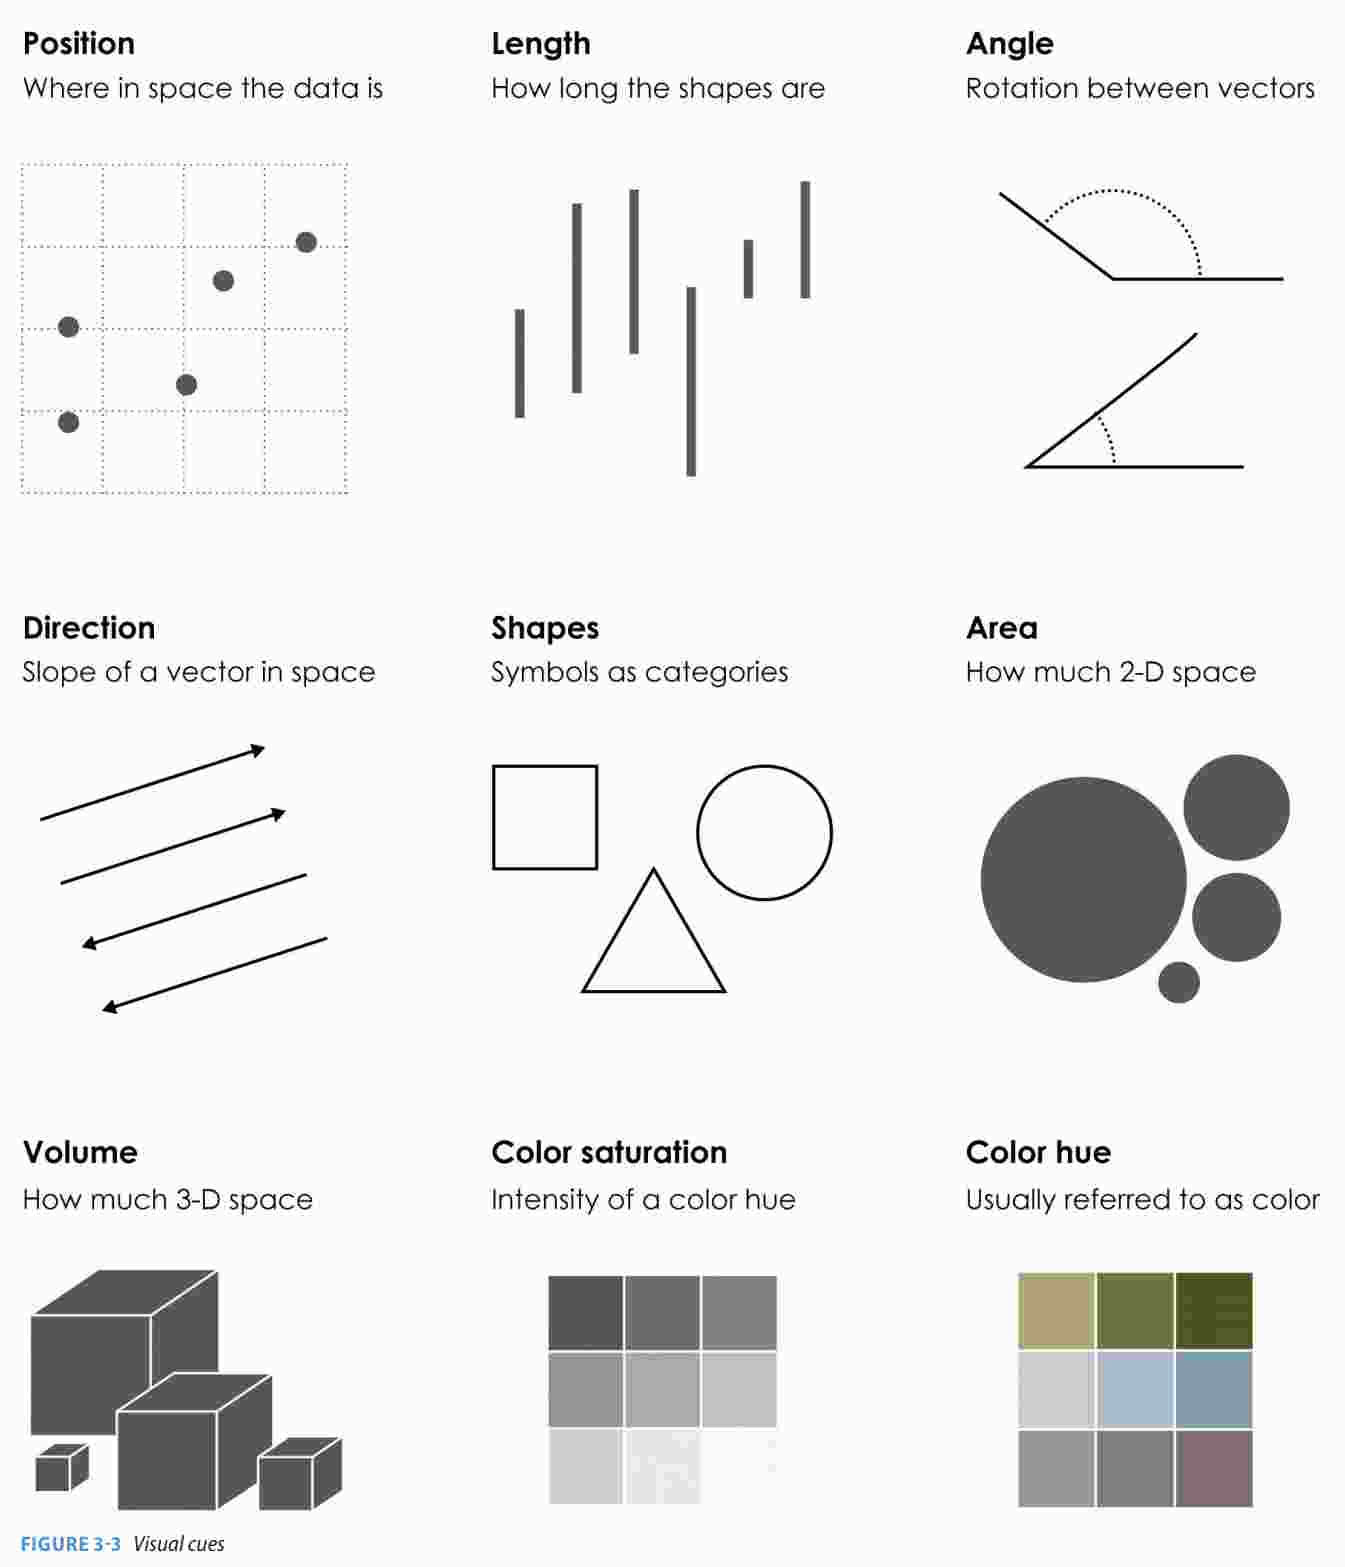
\includegraphics[width=\textwidth]{images/cues} 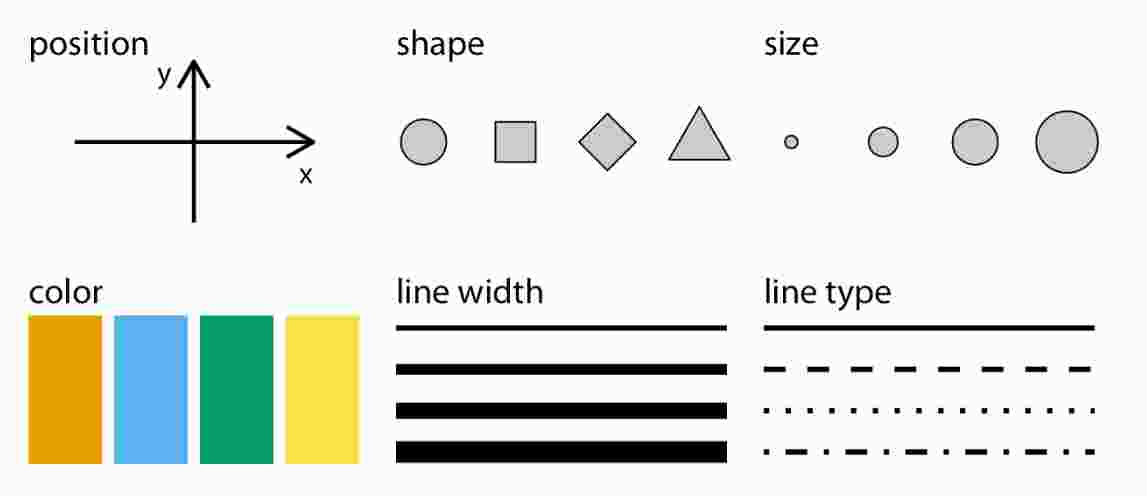
\includegraphics[width=\textwidth]{images/scales} 

}

\caption{Commonly used aesthetics in data visualization.
top: Chapter 3 \citet{Yau}, bottom: Chapter 2 \citet{wilke}}\label{fig:unnamed-chunk-59}
\end{figure}

\section{Coordinate systems}\label{coordinate-systems}

How are the data points organized? While any number of coordinate
systems are possible, three are most common.

\subsection{Cartesian}\label{cartesian}

This is the familiar (\(x, y\))-rectangular coordinate system with two
perpendicular axes.

\subsection{Polar}\label{polar}

The radial analog of the Cartesian system with points identified by
their radius \(\rho\) and angle \(\theta\).

\subsection{Geographic}\label{geographic}

This is the increasingly important system in which we have locations on
the curved surface of the Earth, but we are trying to represent these
locations in a flat two-dimensional plane.




\begin{figure}

{\centering 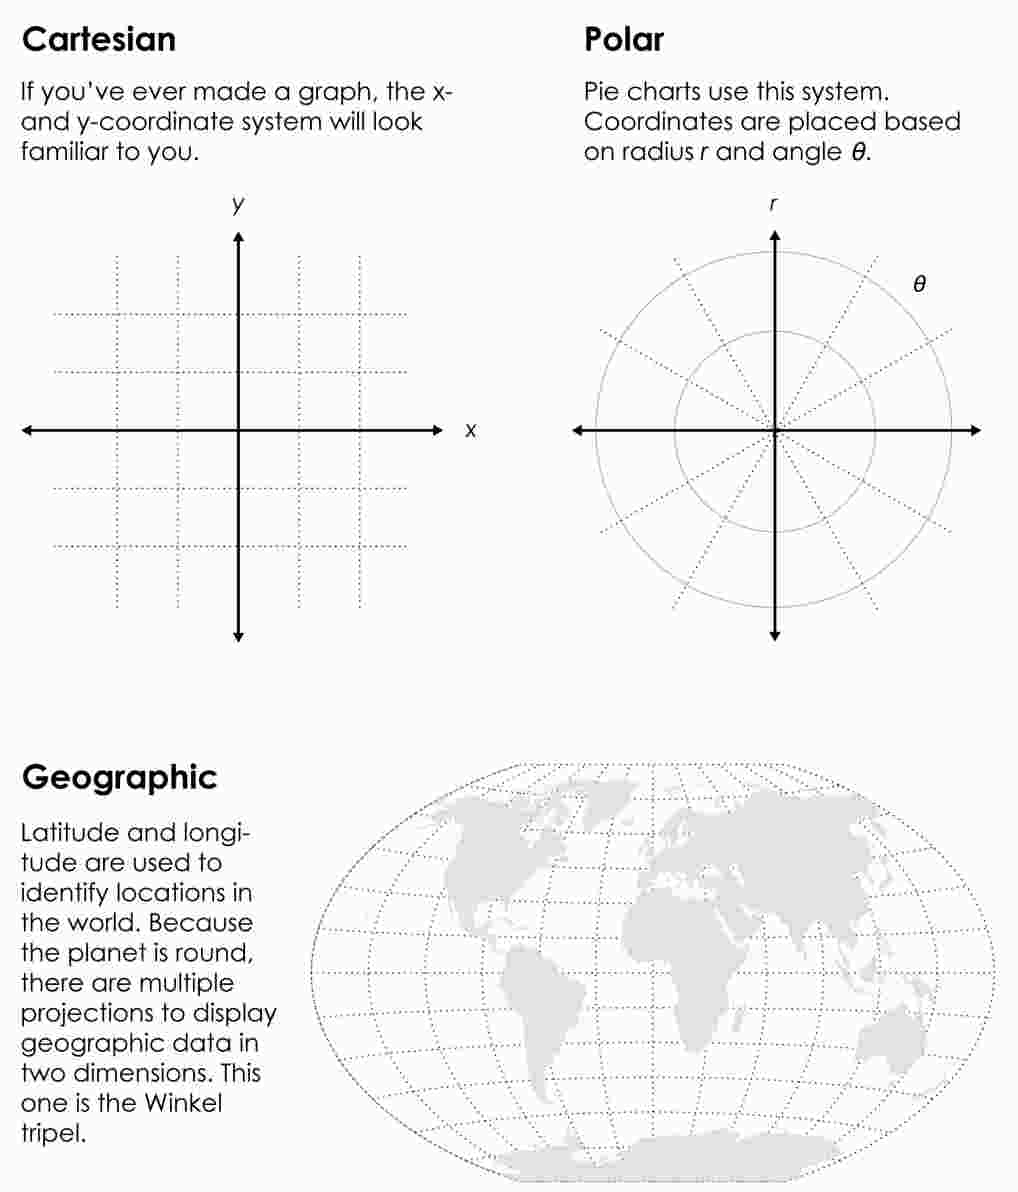
\includegraphics[width=\textwidth]{images/geography} 

}

\caption{Commonly used coordinate systems. Chapter 3
\citet{Yau}.}\label{fig:unnamed-chunk-60}
\end{figure}

\section{Scales}\label{scales}

Scales link data values to aesthetics \citep{wilke}. To map data values
onto aesthetics, we need to specify which data values correspond to
which specific aesthetics values. For example, if our graphic has an x
axis, then we need to specify which data values fall onto particular
positions along this axis. Similarly, we may need to specify which data
values are represented by particular shapes or colors. This mapping
between data values and aesthetics values is created via scales. A scale
defines a unique mapping between data and aesthetics. Importantly, a
scale must be one-to-one, such that for each specific data value there
is exactly one aesthetics value and vice versa. If a scale isn't
one-to-one, then the data visualization becomes ambiguous.






\begin{figure}

{\centering 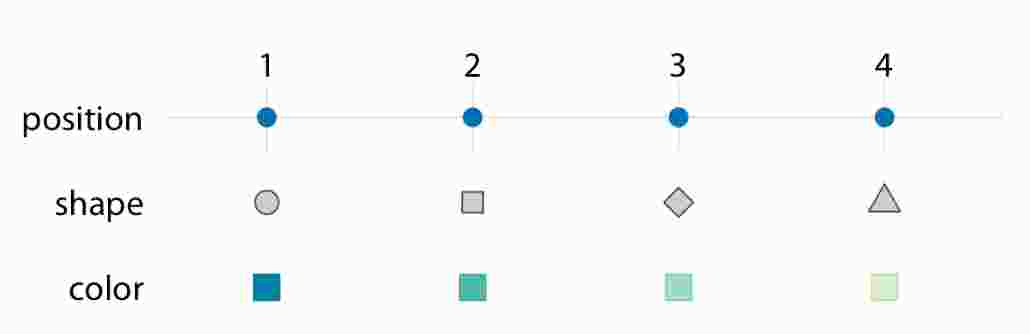
\includegraphics[width=\textwidth]{images/scales2} 

}

\caption{Scales link data values to aesthetics. Here, the numbers 1
through 4 have been mapped onto a position scale, a shape scale, and a
color scale. For each scale, each number corresponds to a unique
position, shape, or color and vice versa \citep{wilke}.}\label{fig:unnamed-chunk-61}
\end{figure}

\section{Context}\label{context}

The purpose of data graphics is to help the viewer make meaningful
comparisons, but a bad data graphic can do just the opposite: It can
instead focus the viewer's attention on meaningless artifacts, or ignore
crucial pieces of relevant but external knowledge. Context can be added
to data graphics in the form of titles or subtitles that explain what is
being shown, axis labels that make it clear how units and scale are
depicted, or reference points or lines that contribute relevant external
information. While one should avoid cluttering up a data graphic with
excessive annotations, it is necessary to provide proper context
\citep{baumer2017mdsr}.

\section{Facets and layers}\label{facets-and-layers}

One of the fundamental challenges of creating data graphics is
condensing multivariate information into a two-dimensional image. While
three-dimensional images are occasionally useful, they are often more
confusing than anything else. Instead, here are three common ways of
incorporating more variables into a two-dimensional data graphic.

\subsection{Facets}\label{facets}

A single data graphic can be composed of several small multiples of the
same basic plot, with one (discrete) variable changing in each of the
small sub-images. An example of facets is shown in Figure \ref{fig:HELP}







\begin{Shaded}
\begin{Highlighting}[]
\NormalTok{pacman}\OperatorTok{::}\KeywordTok{p_load}\NormalTok{(mosaic)}
\KeywordTok{gf_boxplot}\NormalTok{(avg_drinks }\OperatorTok{~}\StringTok{ }\NormalTok{racegrp }\OperatorTok{|}\StringTok{ }\NormalTok{sex, }\DataTypeTok{data =}\NormalTok{ HELPrct)}
\end{Highlighting}
\end{Shaded}

\begin{figure}

{\centering 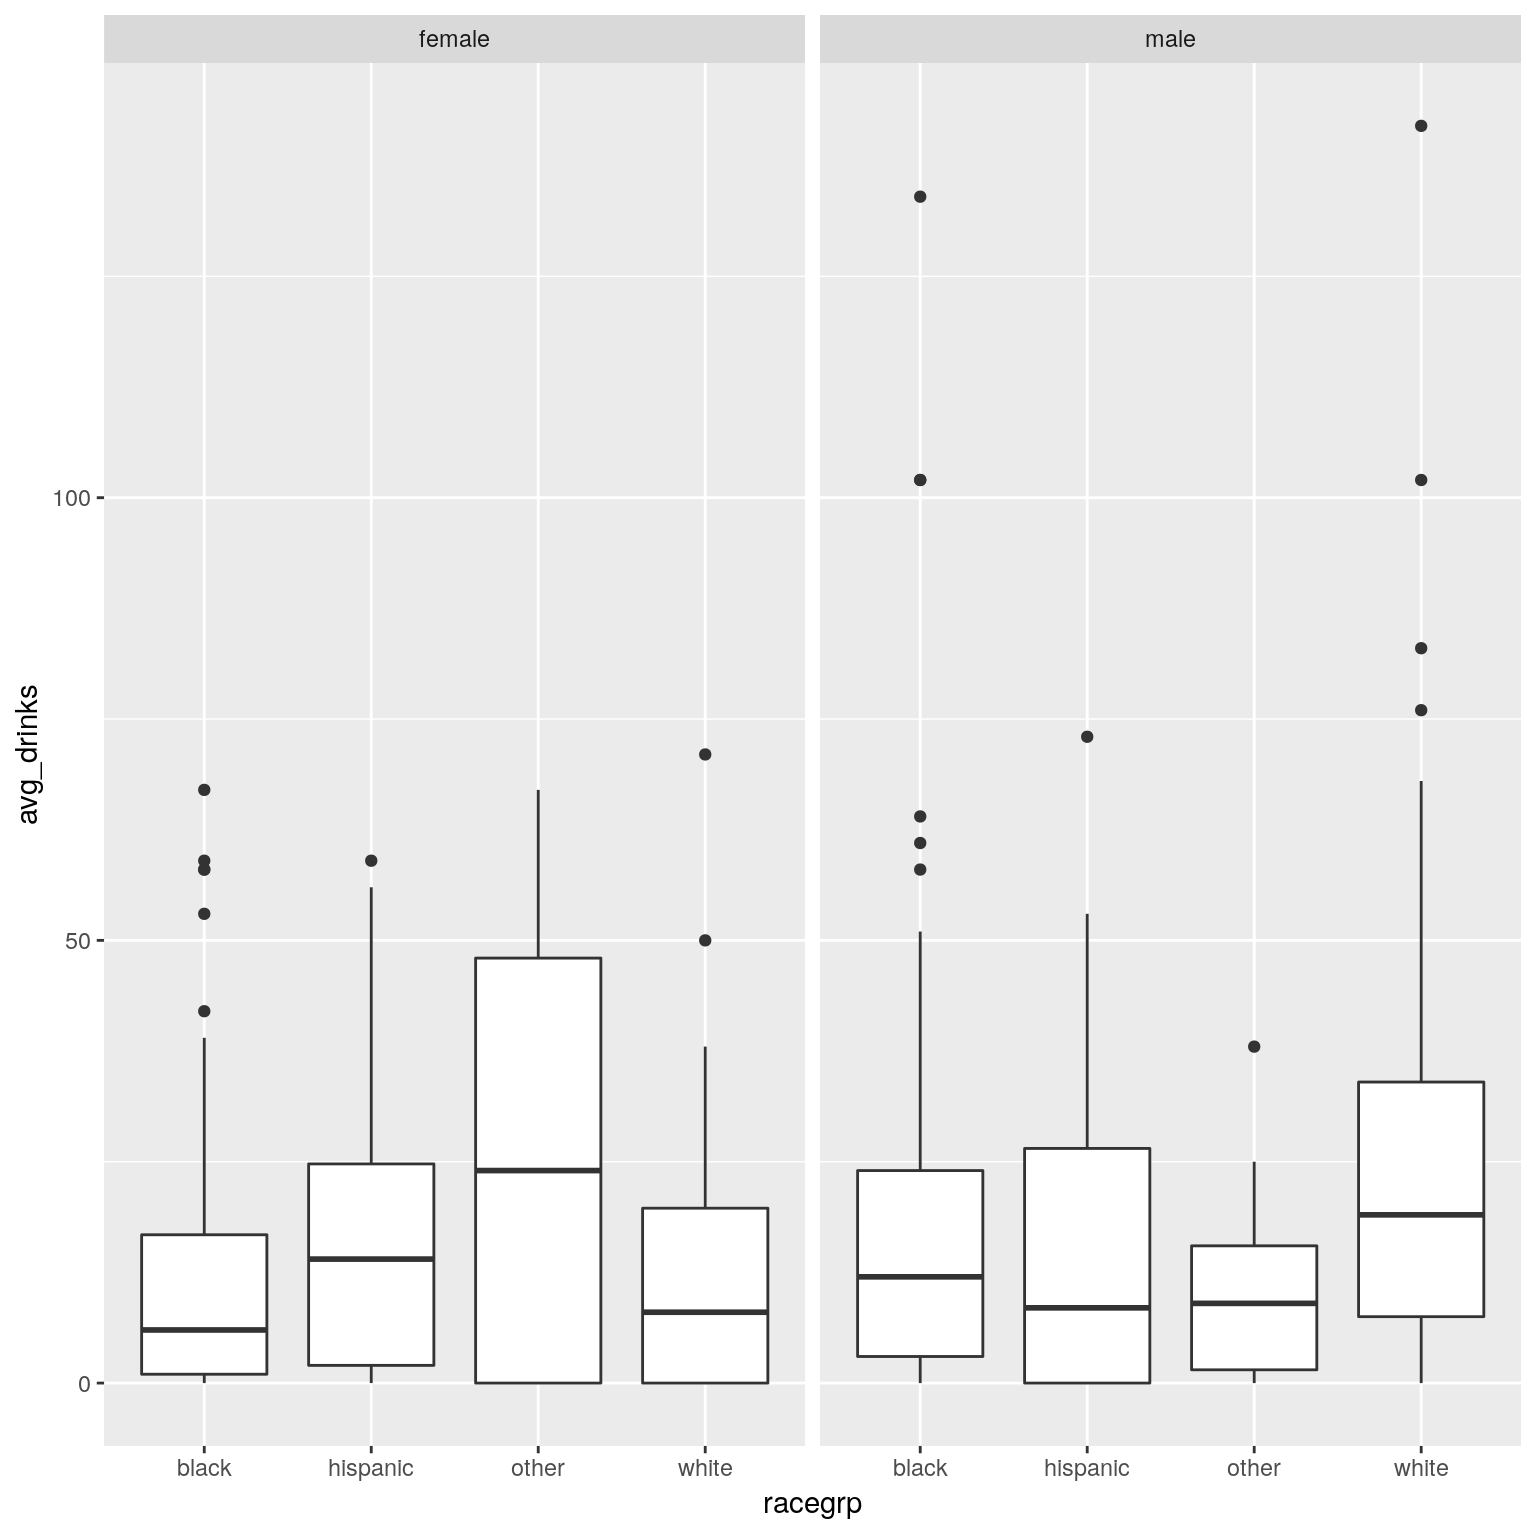
\includegraphics[width=\textwidth]{epib607_files/figure-latex/HELP-1} 

}

\caption{The HELP study was a clinical trial for adult inpatients
recruited from a detoxification unit. Patients with no primary care
physician were randomized to receive a multidisciplinary assessment and
a brief motivational intervention or usual care, with the goal of
linking them to primary medical care.}\label{fig:HELP}
\end{figure}

\subsection{Layers}\label{layers}

It is sometimes appropriate to draw a new layer on top of an existing
data graphic. This new layer can provide context or comparison, but
there is a limit to how many layers humans can reliably parse.

\subsection{Animation}\label{animation}

If time is the additional variable, then an animation can sometimes
effectively convey changes in that variable. Of course, this doesn't
work on the printed page, and makes it impossible for the user to see
all the data at once.

\section{Color}\label{color}

Approximately 8 percent of the population---most of whom are men---have
some form of color blindness. Most commonly, this renders them incapable
of seeing colors accurately, most notably of distinguishing between red
and green. Compounding the problem, many of these people do not know
that they are color-blind. Thus, for professional graphics it is worth
thinking carefully about which colors to use.

Thankfully, we have been freed from the burden of having to create such
intelligent palettes by the research of Cynthia Brewer, creator of the
\href{http://colorbrewer2.org/learnmore/schemes_full.html}{ColorBrewer
website} (and
\href{https://cran.r-project.org/web/packages/RColorBrewer/index.html}{R
package}). Brewer has created colorblind-safe palettes in a variety of
hues for three different types of numeric data in a single variable:

\subsection{Sequential}\label{sequential}

The ordering of the data has only one direction. Positive integers are
sequential because they can only go up: they can't go past 0. (Thus, if
0 is encoded as white, then any darker shade of gray indicates a larger
number.)

\subsection{Diverging}\label{diverging}

The ordering of the data has two directions. In an election forecast, we
com- monly see states colored based on how they are expected to vote for
the president. Since red is associated with Republicans and blue with
Democrats, states that are solidly red or blue are on opposite ends of
the scale. But ``swing states'' that could go either way may appear
purple, white, or some other neutral color that is ``between'' red and
blue.

\subsection{Qualitative}\label{qualitative}

There is no ordering of the data, and we simply need color to
differentiate different categories.

\begin{Shaded}
\begin{Highlighting}[]
\NormalTok{pacman}\OperatorTok{::}\KeywordTok{p_load}\NormalTok{(RColorBrewer)}
\NormalTok{RColorBrewer}\OperatorTok{::}\KeywordTok{display.brewer.all}\NormalTok{()}
\end{Highlighting}
\end{Shaded}

\begin{center}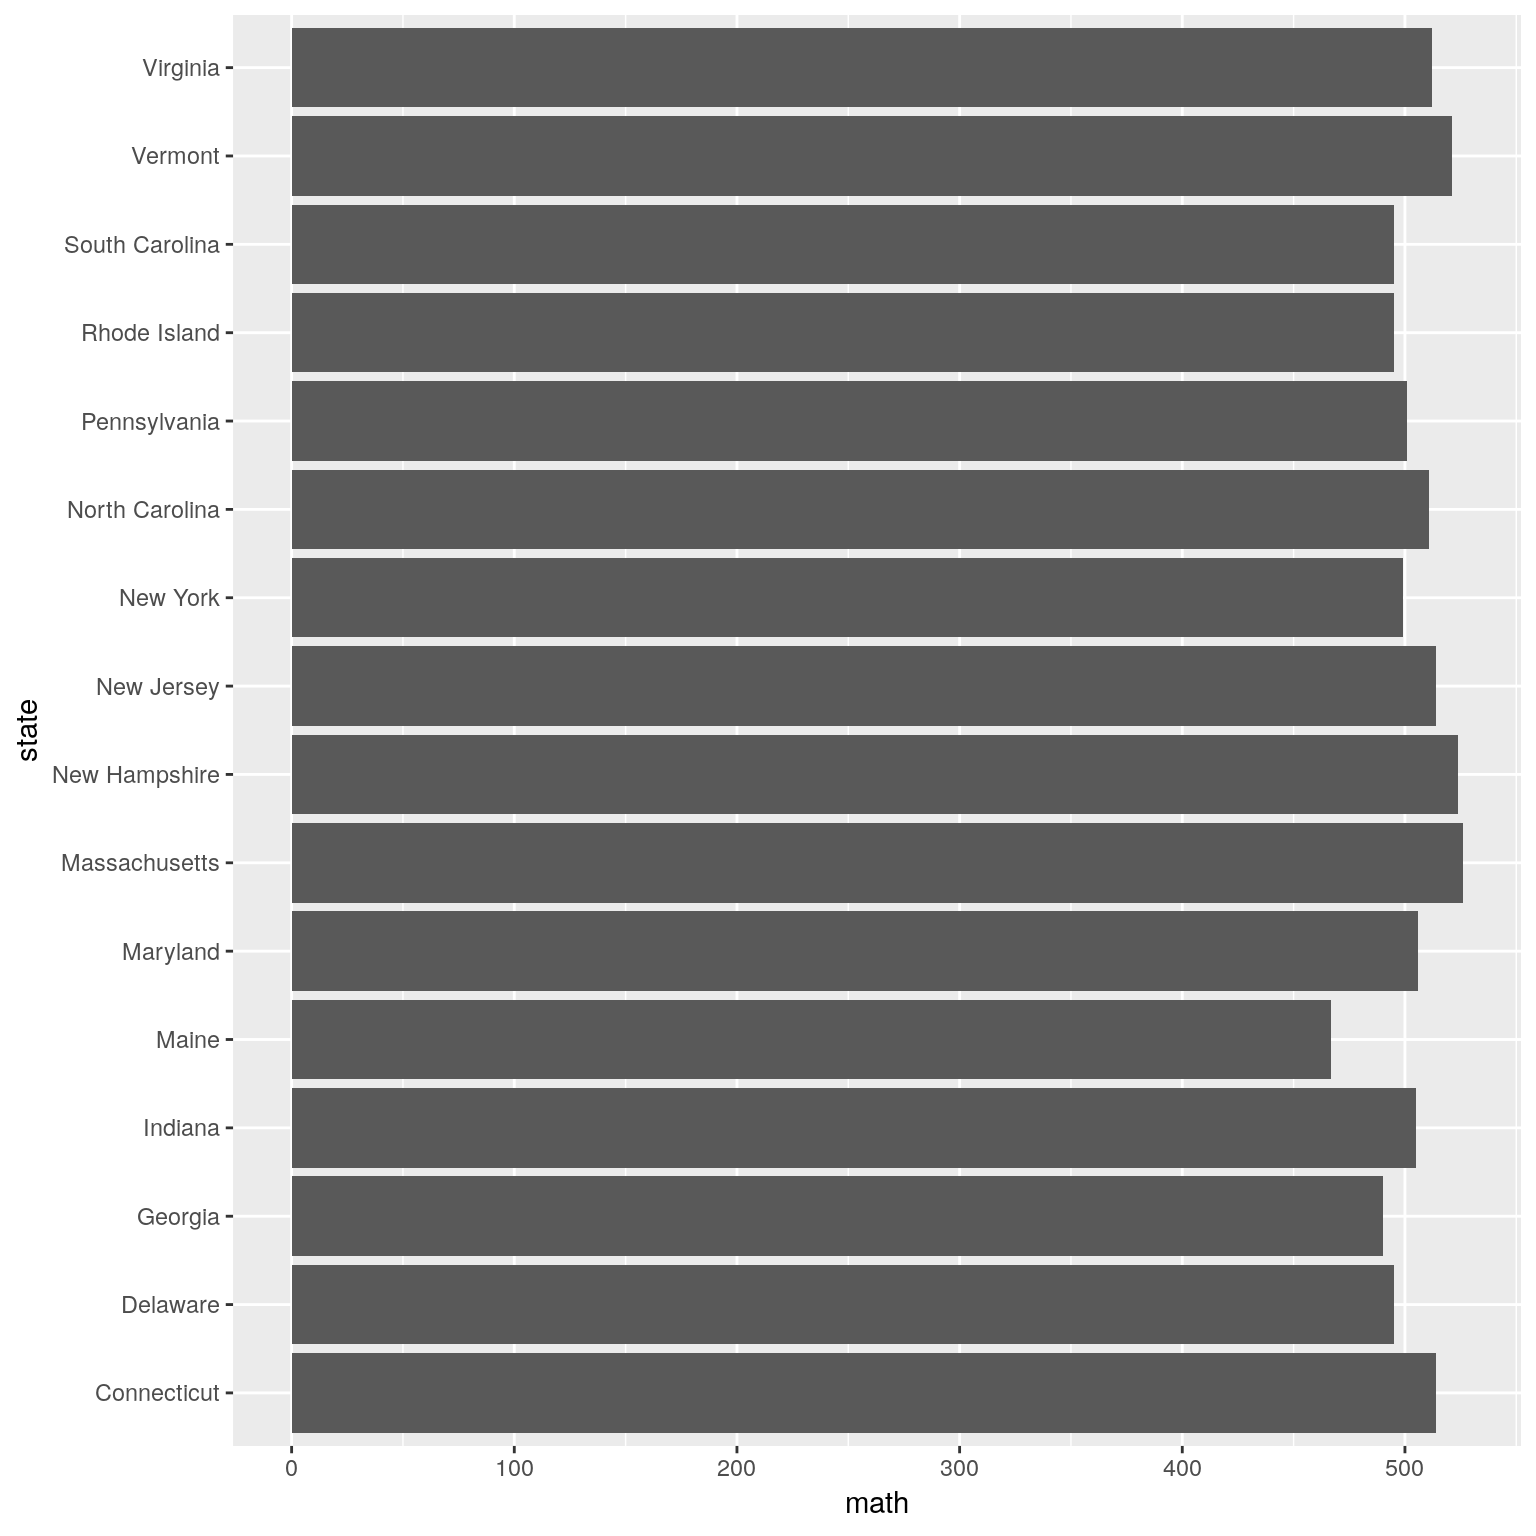
\includegraphics[width=\textwidth]{epib607_files/figure-latex/unnamed-chunk-62-1} \end{center}

Also see the
\href{https://cran.r-project.org/web/packages/viridis/vignettes/intro-to-viridis.html}{viridis
R package} and
\href{https://serialmentor.com/dataviz/color-basics.html}{the Color
Scales chapter} \citep{wilke}.

\section{Examples}\label{examples}

\subsection{Hurricane Florence}\label{hurricane-florence}

For Hurricane Florence, \citet{ncar} present the first advance
forecasted attribution statements about the human influence on a
tropical cyclone. In Figure \ref{fig:ncar} they present a side-by-side
comparison of the rainfall based on two forecasts:

\begin{enumerate}
\def\labelenumi{\arabic{enumi}.}
\tightlist
\item
  \textbf{Standard Forecast}: With observed initial atmospheric
  conditions and sea surface temperatures (SST) adapted from NOAA's
  operational Global Forecast System model. This is the forecast of the
  actual Hurricane Florence.
\item
  \textbf{Modified Forecast}: With observed initial conditions modified
  to remove the estimated climate change signal from the temperature,
  moisture, and SST fields to represent a world without climate change.
  This is a counterfactual forecast of Hurricane Florence if it were to
  occur in a world without human induced global warming.
\end{enumerate}





\begin{figure}

{\centering 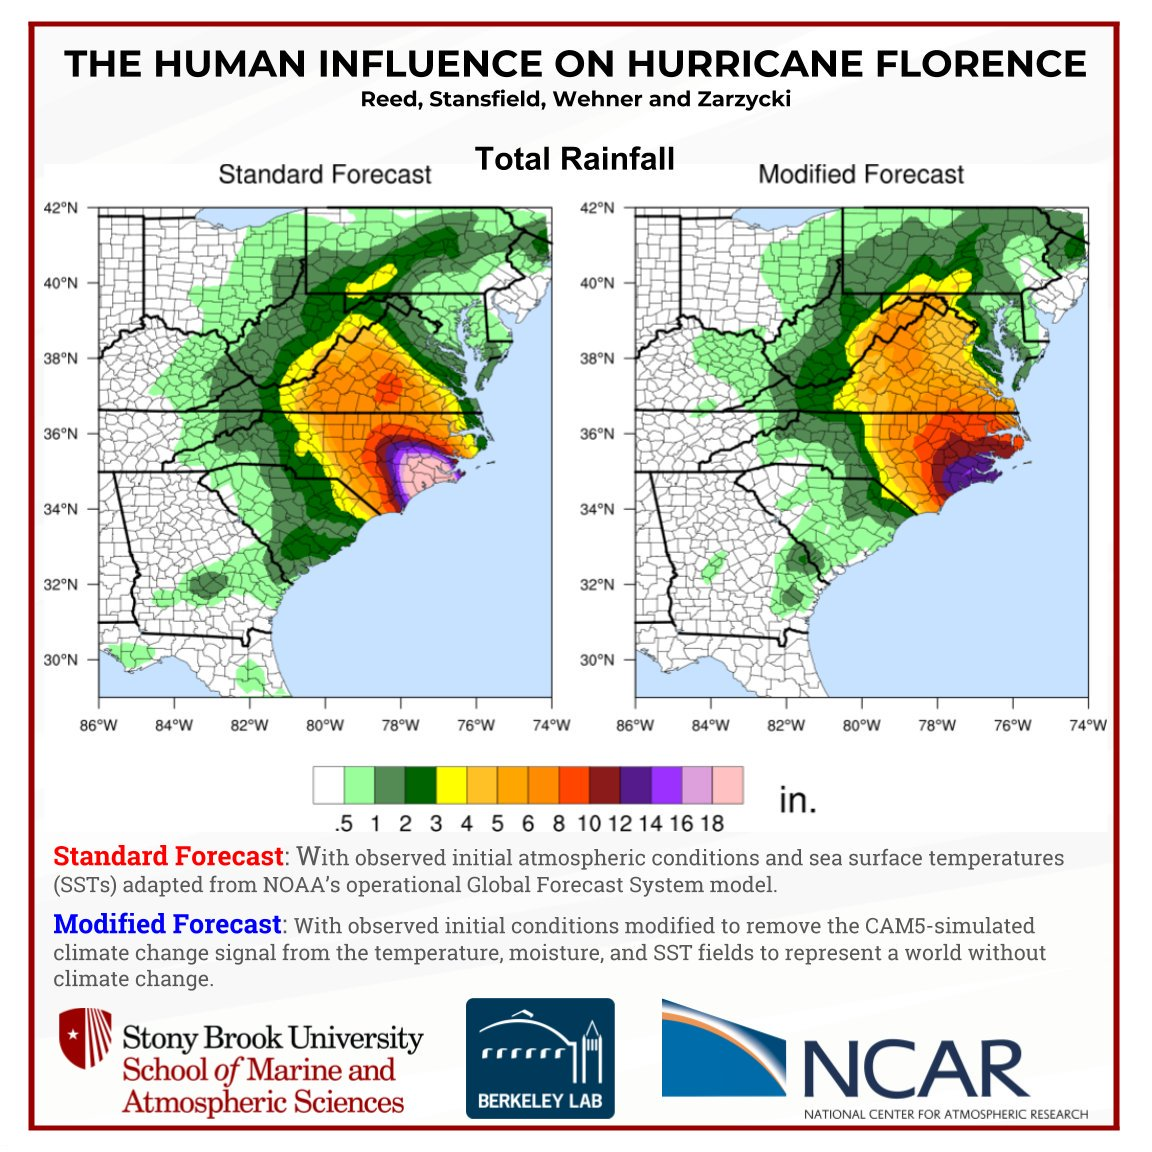
\includegraphics[width=\textwidth]{images/ncar_florence} 

}

\caption{Left: is the forecast of the actual Hurricane Florence.
Right: counterfactual forecast of Hurricane Florence if it were to occur
in a world without human induced global warming \citep{ncar}.}\label{fig:ncar}
\end{figure}

The image on the right (modified forecast) looks worse, but the
situation described on the left (standard forecast) is actually worse.
They should have instead used perceptually uniform sequential colormaps
as shown in Figure \ref{fig:viridis}



\begin{figure}

{\centering 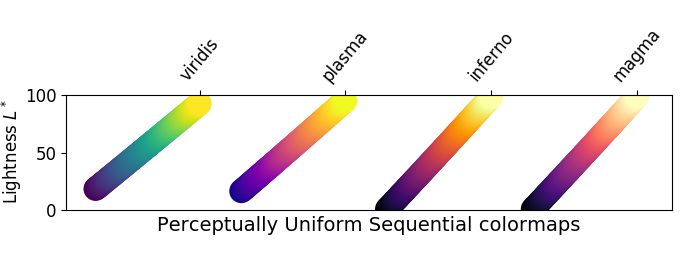
\includegraphics[width=\textwidth]{images/viridis} 

}

\caption{source: \url{https://matplotlib.org/users/colormaps.html}}\label{fig:viridis}
\end{figure}

These palettes are available in \texttt{R} through the
\href{https://cran.r-project.org/web/packages/viridis/vignettes/intro-to-viridis.html}{viridis
R package}.

\subsection{SAT Scores}\label{sat-scores}

The bar graph below displays the average score on the math portion of
the 2010 SAT (with possible scores ranging from 200 to 800) among states
for whom at least two-thirds of the students took the SAT.

\begin{Shaded}
\begin{Highlighting}[]
\NormalTok{pacman}\OperatorTok{::}\KeywordTok{p_load}\NormalTok{(mdsr)}
\NormalTok{pacman}\OperatorTok{::}\KeywordTok{p_load}\NormalTok{(mosaic)}
\KeywordTok{gf_colh}\NormalTok{(state }\OperatorTok{~}\StringTok{ }\NormalTok{math, }\DataTypeTok{data =} \KeywordTok{subset}\NormalTok{(SAT_}\DecValTok{2010}\NormalTok{, sat_pct }\OperatorTok{>}\StringTok{ }\DecValTok{66}\NormalTok{)) }
\end{Highlighting}
\end{Shaded}

\begin{center}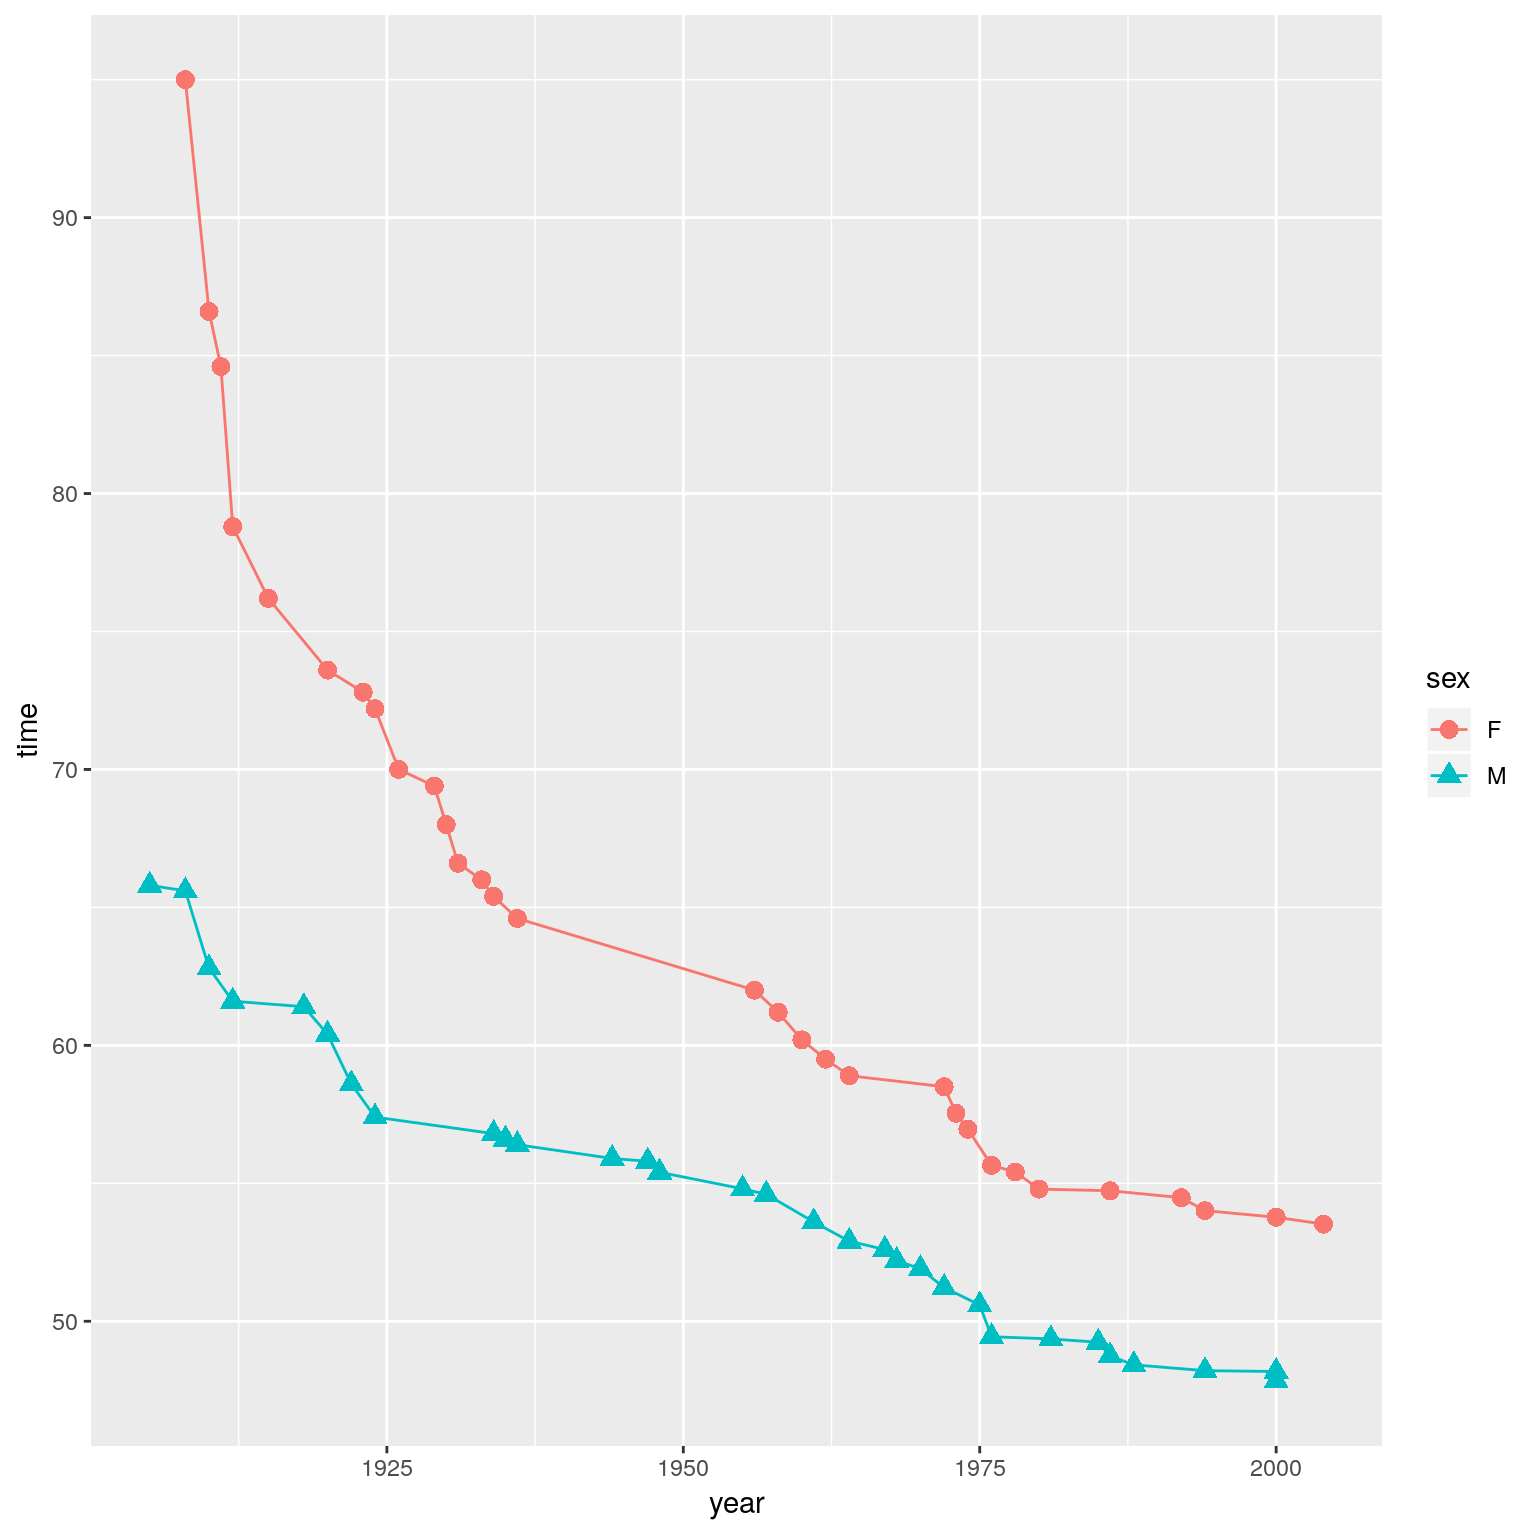
\includegraphics[width=\textwidth]{epib607_files/figure-latex/unnamed-chunk-63-1} \end{center}

This plot uses the visual cue of position to represent the math SAT
score on the vertical axis with. The categorical variable of state is
arrayed on the horizontal axis. It would not be appropriate to consider
the state variable to be ordinal, since the ordering is not meaningful
in the context of math SAT scores. The coordinate system is Cartesian,
although as noted previously, the horizontal coordinate is meaningless.
Context is provided by the axis labels and title.

\subsection{Swimming records}\label{swimming-records}

Next, we consider a time series that shows the progression of the world
record times in the 100-meter freestyle swimming event for men and
women. The Figure below displays the times as a function of the year in
which the new record was set. At some level this is simply a scatterplot
that uses position on both the vertical and horizontal axes to indicate
swimming time and chronological time, respectively, in a Cartesian
plane. The numeric scale on the vertical axis is linear, in units of
seconds, while the scale on the horizontal axis is also linear, measured
in years. But there is more going on here. Color is being used as a
visual cue to distinguish the categorical variable sex. Furthermore,
since the points are connected by lines, direction is being used to
indicate the progression of the record times. (In this case, the records
can only get faster, so the direction is always down.) One might even
argue that angle is being used to compare the descent of the world
records across time and/or gender. In fact, in this case shape is also
being used to distinguish sex.

\begin{Shaded}
\begin{Highlighting}[]
\NormalTok{pacman}\OperatorTok{::}\KeywordTok{p_load}\NormalTok{(mosaicData)}
\KeywordTok{gf_point}\NormalTok{(time }\OperatorTok{~}\StringTok{ }\NormalTok{year , }\DataTypeTok{data =}\NormalTok{ SwimRecords, }\DataTypeTok{color =} \OperatorTok{~}\StringTok{ }\NormalTok{sex, }\DataTypeTok{shape =} \OperatorTok{~}\StringTok{ }\NormalTok{sex, }\DataTypeTok{size =} \DecValTok{3}\NormalTok{) }\OperatorTok\StringTok{ }
\StringTok{  }\KeywordTok{gf_line}\NormalTok{(time }\OperatorTok{~}\StringTok{ }\NormalTok{year , }\DataTypeTok{data =}\NormalTok{ SwimRecords, }\DataTypeTok{color =} \OperatorTok{~}\StringTok{ }\NormalTok{sex)}
\end{Highlighting}
\end{Shaded}

\begin{center}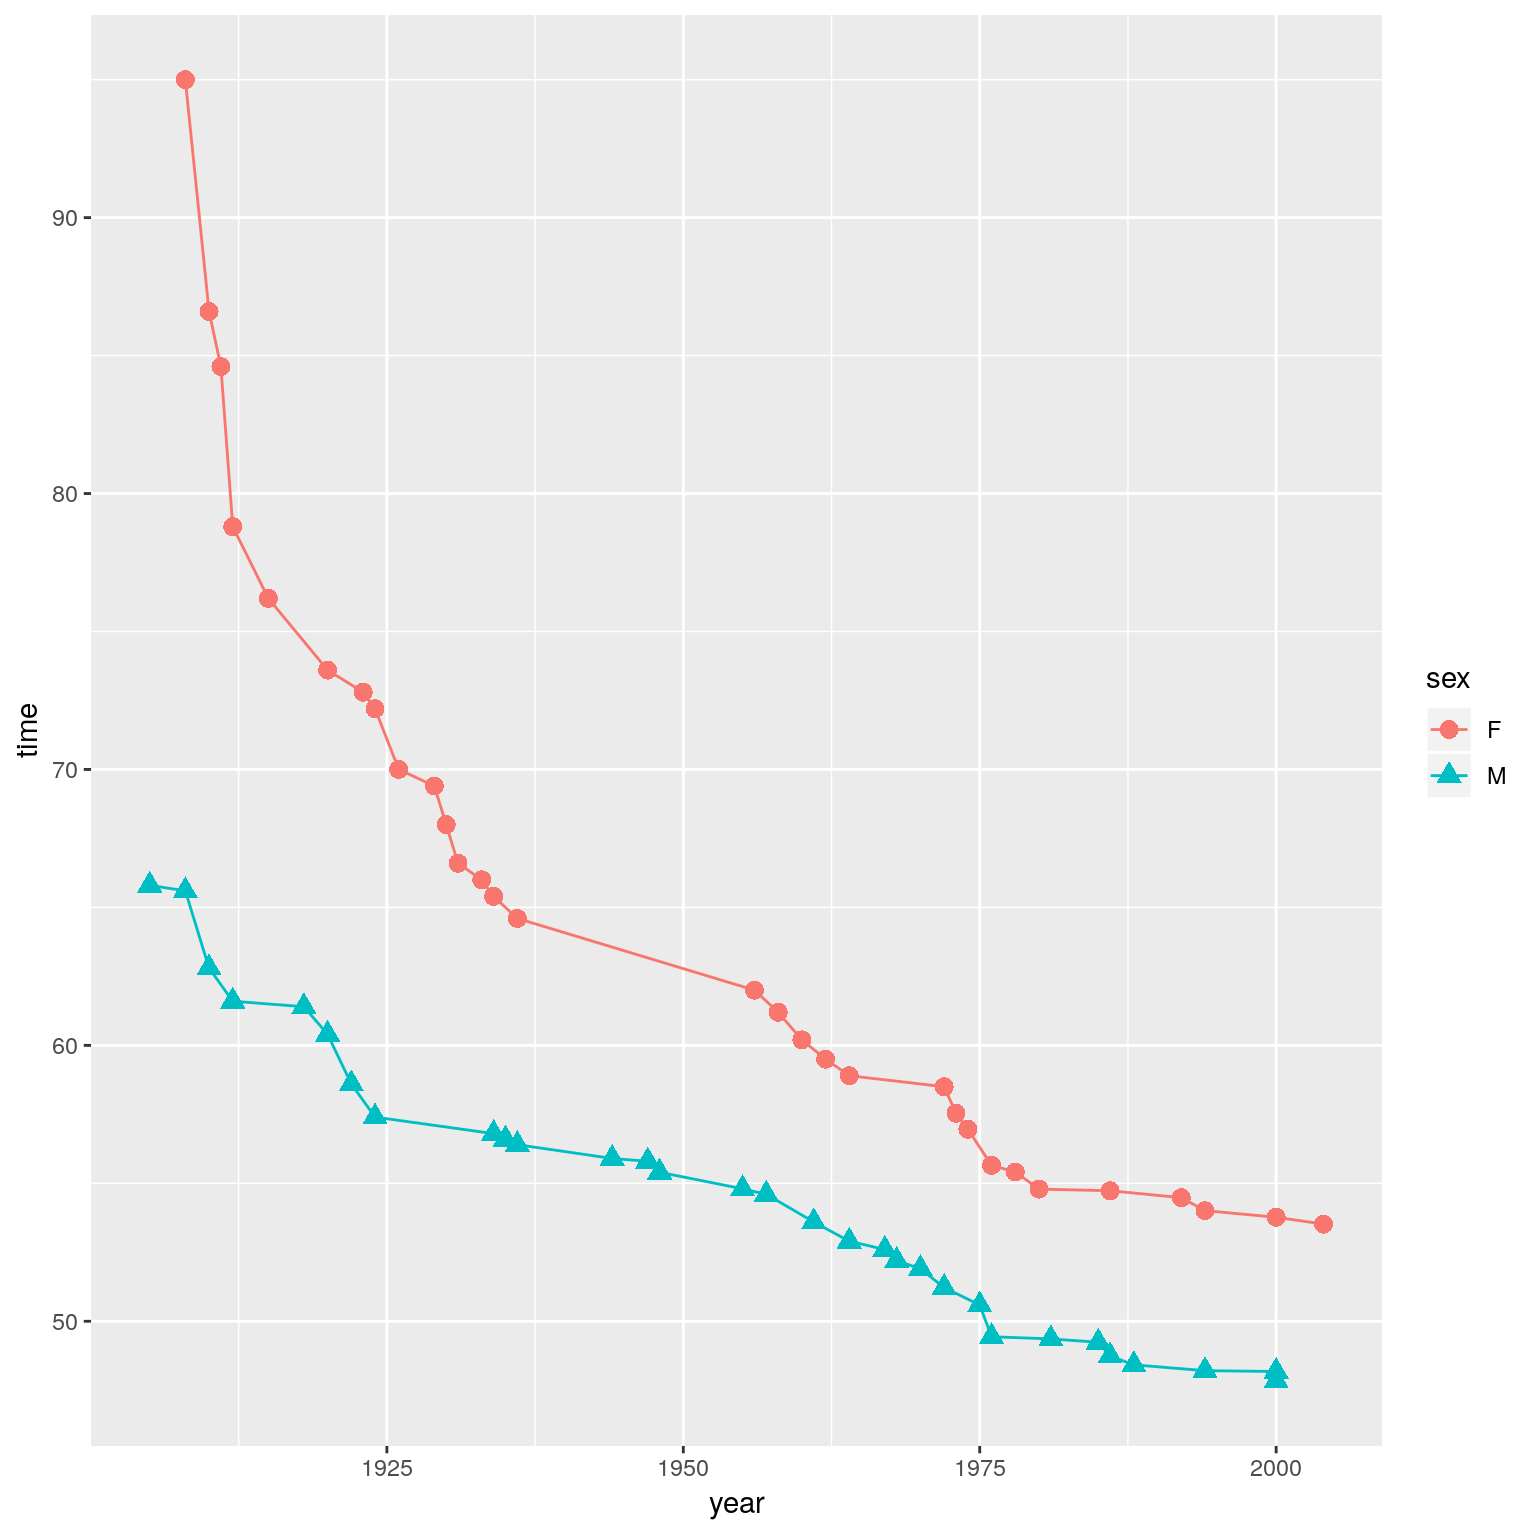
\includegraphics[width=\textwidth]{epib607_files/figure-latex/unnamed-chunk-64-1} \end{center}

\section{Exercises}\label{exercises}

\subsection{Exercise 1}\label{exercise-1}

For this exercise, refer to the article assigned to your team in the
\href{https://sahirbhatnagar.com/EPIB607/terms-and-concepts.html}{Terms
and Concepts} exercise.

\begin{enumerate}
\def\labelenumi{\arabic{enumi}.}
\tightlist
\item
  Identify the aesthetics and scale(s). If your article did not contain
  a graphic, pick a Table in your paper and think about what graphic
  could have been used instead. See
  \href{https://serialmentor.com/dataviz/directory-of-visualizations.html}{Fundamentals
  of Data Visualization} and
  \href{http://r-statistics.co/Top50-Ggplot2-Visualizations-MasterList-R-Code.html\#1.\%20Correlation}{Top
  50 ggplot2 Visualizations} for examples of graphics.
\item
  How many variables are depicted in the graphic? Explicitly link each
  variable to an aesthetic that you listed above.
\item
  Critique this data graphic using the taxonomy described in this
  chapter.
\end{enumerate}

\subsection{Exercise 2}\label{exercise-2}

Vox published a list of
\href{http://www.vox.com/a/explain-food-america}{Charts that explain
food in America}. There are 40 maps, charts, and graphs that show where
our food and drink comes from and how we eat it.

Pick your best and least favorite graphic. One representative from each
group will present in 1 minute or less their rationale for the groups
choices.

\appendix


\chapter{Vectorization, *apply and for
loops}\label{vectorization-apply-and-for-loops}

This section will cover the basics of vectorizations, the
\texttt{*apply} family of functions and \texttt{for} loops.

\section{Vectorization}\label{vectorization}

Almost everything in \texttt{R} is a vector. A scalar is really a vector
of length 1 and a \texttt{data.frame} is a collection of vectors. An
nice feature of \texttt{R} is its vectorized capabilities. Vectorization
indicates that a function operates on a whole vector of values at the
same time and not just on a single value\footnote{\url{http://www.dummies.com/how-to/content/how-to-vectorize-your-functions-in-r.html}}.
If you have have ever taken a basic linear algebra course, this concept
will be familiar to you. \newline  \vspace{0.1in} Take for example two
vectors: \newline
\vspace{0.1in} \[
\begin{bmatrix} 1 \\ 2 \\ 3 \end{bmatrix} + 
\begin{bmatrix} 1 \\ 2 \\ 3 \end{bmatrix} =
\begin{bmatrix} 2 \\ 4 \\ 6 \end{bmatrix}
\] \newline  \vspace{0.1in} The corresponding \texttt{R} code is given
by:

\begin{Shaded}
\begin{Highlighting}[]
\NormalTok{a <-}\StringTok{ }\KeywordTok{c}\NormalTok{(}\DecValTok{1}\NormalTok{,}\DecValTok{2}\NormalTok{,}\DecValTok{3}\NormalTok{)}
\NormalTok{b <-}\StringTok{ }\KeywordTok{c}\NormalTok{(}\DecValTok{1}\NormalTok{,}\DecValTok{2}\NormalTok{,}\DecValTok{3}\NormalTok{)}
\NormalTok{a}\OperatorTok{+}\NormalTok{b}
\CommentTok{#> [1] 2 4 6}
\end{Highlighting}
\end{Shaded}

Many of the \texttt{base} functions in \texttt{R} are already
vectorized. Here are some common examples:

\begin{Shaded}
\begin{Highlighting}[]

\CommentTok{# generate a sequence of numbers from 1 to 10}
\NormalTok{(a <-}\StringTok{ }\DecValTok{1}\OperatorTok{:}\DecValTok{10}\NormalTok{)}
\CommentTok{#>  [1]  1  2  3  4  5  6  7  8  9 10}

\CommentTok{# sum the numbers from 1 to 10}
\KeywordTok{sum}\NormalTok{(a)}
\CommentTok{#> [1] 55}

\CommentTok{# calculate sums of each column}
\KeywordTok{colSums}\NormalTok{(iris[, }\OperatorTok{-}\DecValTok{5}\NormalTok{])}
\CommentTok{#> Sepal.Length  Sepal.Width Petal.Length  Petal.Width }
\CommentTok{#>        876.5        458.6        563.7        179.9}
\end{Highlighting}
\end{Shaded}

\begin{quote}
\textbf{Exercise}: What happens when you sum two vectors of different
lengths?
\end{quote}

\section{\texorpdfstring{Family of \texttt{*apply}
functions}{Family of *apply functions}}\label{family-of-apply-functions}

\begin{itemize}
\tightlist
\item
  \texttt{apply}, \texttt{lapply} and \texttt{sapply} are some of the
  most commonly used class of functions in \texttt{R}
\item
  \texttt{*apply} functions are not necessarily faster than loops, but
  can be easier to read (and vice cersa)
\item
  \texttt{apply} is used when you need to perform an operation on every
  row or column of a matrix or data.frame
\item
  \texttt{lapply} and \texttt{sapply} differ in the format of the
  output. The former returns a list while the ladder returns a vector
\item
  There are other \texttt{*apply} functions such as \texttt{tapply},
  \texttt{vapply} and \texttt{mapply} with similar functionality and
  purpose
\end{itemize}

\subsection{Loops vs.~Apply}\label{loops-vs.apply}

\begin{Shaded}
\begin{Highlighting}[]

\CommentTok{# Getting the row means of two columns}
\CommentTok{# Generate data}
\NormalTok{N <-}\StringTok{ }\DecValTok{10000}
\NormalTok{x1 <-}\StringTok{ }\KeywordTok{runif}\NormalTok{(N)}
\NormalTok{x2 <-}\StringTok{ }\KeywordTok{runif}\NormalTok{(N)}
\NormalTok{d <-}\StringTok{ }\KeywordTok{as.data.frame}\NormalTok{(}\KeywordTok{cbind}\NormalTok{(x1, x2))}
\KeywordTok{head}\NormalTok{(d)}
\CommentTok{#>        x1     x2}
\CommentTok{#> 1 0.57632 0.9615}
\CommentTok{#> 2 0.56474 0.1950}
\CommentTok{#> 3 0.07399 0.3001}
\CommentTok{#> 4 0.45387 0.3823}
\CommentTok{#> 5 0.37328 0.1197}
\CommentTok{#> 6 0.33132 0.9891}

\CommentTok{# Loop:}
\CommentTok{# create a vector to store the results in }
\NormalTok{rowMeanFor <-}\StringTok{ }\KeywordTok{vector}\NormalTok{(}\StringTok{"double"}\NormalTok{, N)}

\ControlFlowTok{for}\NormalTok{ (i }\ControlFlowTok{in} \KeywordTok{seq_len}\NormalTok{(N)) \{}
\NormalTok{        rowMeanFor[[i]] <-}\StringTok{ }\KeywordTok{mean}\NormalTok{(}\KeywordTok{c}\NormalTok{(d[i, }\DecValTok{1}\NormalTok{], d[i, }\DecValTok{2}\NormalTok{]))}
\NormalTok{\}}

\CommentTok{# Apply:}
\NormalTok{rowMeanApply <-}\StringTok{ }\KeywordTok{apply}\NormalTok{(d, }\DecValTok{1}\NormalTok{, mean)}

\CommentTok{# are the results equal}
\KeywordTok{all.equal}\NormalTok{(rowMeanFor,rowMeanApply)}
\CommentTok{#> [1] TRUE}
\end{Highlighting}
\end{Shaded}

\subsection{\texorpdfstring{Descriptive Statistics using
\texttt{*apply}}{Descriptive Statistics using *apply}}\label{descriptive-statistics-using-apply}

\begin{Shaded}
\begin{Highlighting}[]
\KeywordTok{data}\NormalTok{(women)}
\CommentTok{# data structure}
\KeywordTok{str}\NormalTok{(women)}
\CommentTok{#> 'data.frame':    15 obs. of  2 variables:}
\CommentTok{#>  $ height: num  58 59 60 61 62 63 64 65 66 67 ...}
\CommentTok{#>  $ weight: num  115 117 120 123 126 129 132 135 139 142 ...}

\CommentTok{# calculate the mean for each column}
\KeywordTok{apply}\NormalTok{(women, }\DecValTok{2}\NormalTok{, mean)}
\CommentTok{#> height weight }
\CommentTok{#>   65.0  136.7}

\CommentTok{# apply 'fivenum' function to each column}
\KeywordTok{vapply}\NormalTok{(women, fivenum, }\KeywordTok{c}\NormalTok{(}\StringTok{"Min."}\NormalTok{ =}\StringTok{ }\DecValTok{0}\NormalTok{, }\StringTok{"1st Qu."}\NormalTok{ =}\StringTok{ }\DecValTok{0}\NormalTok{, }\StringTok{"Median"}\NormalTok{ =}\StringTok{ }\DecValTok{0}\NormalTok{, }
                         \StringTok{"3rd Qu."}\NormalTok{ =}\StringTok{ }\DecValTok{0}\NormalTok{, }\StringTok{"Max."}\NormalTok{ =}\StringTok{ }\DecValTok{0}\NormalTok{))}
\CommentTok{#>         height weight}
\CommentTok{#> Min.      58.0  115.0}
\CommentTok{#> 1st Qu.   61.5  124.5}
\CommentTok{#> Median    65.0  135.0}
\CommentTok{#> 3rd Qu.   68.5  148.0}
\CommentTok{#> Max.      72.0  164.0}
\end{Highlighting}
\end{Shaded}

\subsection{\texorpdfstring{Creating new columns using
\texttt{sapply}}{Creating new columns using sapply}}\label{creating-new-columns-using-sapply}

You can apply a \emph{user defined function} to columns or the entire
data frame:

\begin{Shaded}
\begin{Highlighting}[]
\CommentTok{# the ouput of sapply is a vector}
\CommentTok{# the 's' in sapply stands for 'simplified' apply}
\NormalTok{mtcars}\OperatorTok{$}\NormalTok{gear2 <-}\StringTok{ }\KeywordTok{sapply}\NormalTok{(mtcars}\OperatorTok{$}\NormalTok{gear, }
                       \ControlFlowTok{function}\NormalTok{(i) }\ControlFlowTok{if}\NormalTok{ (i}\OperatorTok{==}\DecValTok{4}\NormalTok{) }\StringTok{"alot"} \ControlFlowTok{else} \StringTok{"some"}\NormalTok{)}

\KeywordTok{head}\NormalTok{(mtcars)[,}\KeywordTok{c}\NormalTok{(}\StringTok{"gear"}\NormalTok{,}\StringTok{"gear2"}\NormalTok{)]}
\CommentTok{#>                   gear gear2}
\CommentTok{#> Mazda RX4            4  alot}
\CommentTok{#> Mazda RX4 Wag        4  alot}
\CommentTok{#> Datsun 710           4  alot}
\CommentTok{#> Hornet 4 Drive       3  some}
\CommentTok{#> Hornet Sportabout    3  some}
\CommentTok{#> Valiant              3  some}
\end{Highlighting}
\end{Shaded}

\subsection{\texorpdfstring{Applying functions to subsets using
\texttt{tapply}}{Applying functions to subsets using tapply}}\label{applying-functions-to-subsets-using-tapply}

\begin{Shaded}
\begin{Highlighting}[]

\CommentTok{# Fisher's famous dataset }
\KeywordTok{data}\NormalTok{(iris)}
\KeywordTok{str}\NormalTok{(iris)}
\CommentTok{#> 'data.frame':    150 obs. of  5 variables:}
\CommentTok{#>  $ Sepal.Length: num  5.1 4.9 4.7 4.6 5 5.4 4.6 5 4.4 4.9 ...}
\CommentTok{#>  $ Sepal.Width : num  3.5 3 3.2 3.1 3.6 3.9 3.4 3.4 2.9 3.1 ...}
\CommentTok{#>  $ Petal.Length: num  1.4 1.4 1.3 1.5 1.4 1.7 1.4 1.5 1.4 1.5 ...}
\CommentTok{#>  $ Petal.Width : num  0.2 0.2 0.2 0.2 0.2 0.4 0.3 0.2 0.2 0.1 ...}
\CommentTok{#>  $ Species     : Factor w/ 3 levels "setosa","versicolor",..: 1 1 1 1 1 1 1 1 1 1 ...}

\CommentTok{# mean sepal length by species }
\KeywordTok{tapply}\NormalTok{(iris}\OperatorTok{$}\NormalTok{Sepal.Length, iris}\OperatorTok{$}\NormalTok{Species, mean)}
\CommentTok{#>     setosa versicolor  virginica }
\CommentTok{#>      5.006      5.936      6.588}
\end{Highlighting}
\end{Shaded}

\subsection{\texorpdfstring{Nested for loops using
\texttt{mapply}}{Nested for loops using mapply}}\label{nested-for-loops-using-mapply}

\texttt{mapply} is my favorite \texttt{base} \texttt{R} function and
here are some reasons why:

\begin{itemize}
\tightlist
\item
  Using \texttt{mapply} is equivalent to writing nested \texttt{for}
  loops except that it is 100\% more human readable and less prone to
  errors
\item
  It is an effective way of conducting simulations because it iterates
  of many arguments
\end{itemize}

Let's say you want to generate random samples from a normal distribution
with varying means and standard deviations. Of course the brute force
way would be to write out the command once, copy paste as many times as
you want, and then manually change the arguments for \texttt{mean} and
\texttt{sd} in the \texttt{rnorm} function as so:

\begin{Shaded}
\begin{Highlighting}[]
\NormalTok{v1 <-}\StringTok{ }\KeywordTok{rnorm}\NormalTok{(}\DecValTok{100}\NormalTok{, }\DataTypeTok{mean =} \DecValTok{5}\NormalTok{, }\DataTypeTok{sd =} \DecValTok{1}\NormalTok{)}
\NormalTok{v2 <-}\StringTok{ }\KeywordTok{rnorm}\NormalTok{(}\DecValTok{100}\NormalTok{, }\DataTypeTok{mean =} \DecValTok{10}\NormalTok{, }\DataTypeTok{sd =} \DecValTok{5}\NormalTok{)}
\NormalTok{v3 <-}\StringTok{ }\KeywordTok{rnorm}\NormalTok{(}\DecValTok{100}\NormalTok{, }\DataTypeTok{mean =} \OperatorTok{-}\DecValTok{3}\NormalTok{, }\DataTypeTok{sd =} \DecValTok{10}\NormalTok{)}
\end{Highlighting}
\end{Shaded}

This isn't too bad for three vectors. But what if you want to generate
many more combinations of means and sds ? Furthermore, how can you keep
track of the parameters you used? Now lets consider the \texttt{mapply}
function:

\begin{Shaded}
\begin{Highlighting}[]
\NormalTok{means <-}\StringTok{ }\KeywordTok{c}\NormalTok{(}\DecValTok{5}\NormalTok{,}\DecValTok{10}\NormalTok{,}\OperatorTok{-}\DecValTok{3}\NormalTok{) ; sds <-}\StringTok{ }\KeywordTok{c}\NormalTok{(}\DecValTok{1}\NormalTok{,}\DecValTok{5}\NormalTok{,}\DecValTok{10}\NormalTok{) }

\CommentTok{# MoreArgs is a list of arguments that dont change}
\NormalTok{randomNormals <-}\StringTok{ }\KeywordTok{mapply}\NormalTok{(rnorm, }\DataTypeTok{mean =}\NormalTok{ means, }\DataTypeTok{sd =}\NormalTok{ sds, }
                        \DataTypeTok{MoreArgs =} \KeywordTok{list}\NormalTok{(}\DataTypeTok{n =} \DecValTok{100}\NormalTok{))}

\KeywordTok{head}\NormalTok{(randomNormals)}
\CommentTok{#>       [,1]   [,2]    [,3]}
\CommentTok{#> [1,] 3.836  8.771   5.144}
\CommentTok{#> [2,] 4.525  9.376  -2.280}
\CommentTok{#> [3,] 4.072 13.144   2.940}
\CommentTok{#> [4,] 4.737 18.210 -13.118}
\CommentTok{#> [5,] 5.690 22.951  -7.008}
\CommentTok{#> [6,] 4.826  7.615 -15.323}
\end{Highlighting}
\end{Shaded}

The following diagram (from
\href{http://r4ds.had.co.nz/iteration.html\#mapping-over-multiple-arguments}{r4ds})
describes exactly what is going on in the above function call to
\texttt{mapply}:

\begin{figure}
\centering
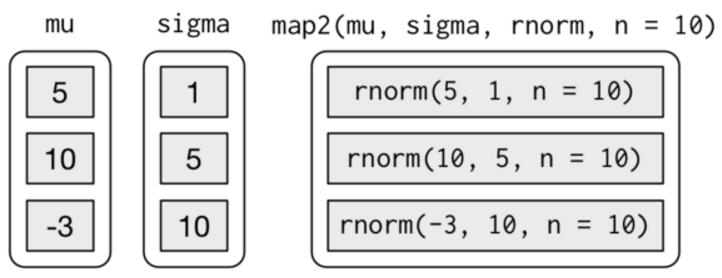
\includegraphics{images/mapply.png}
\caption{}
\end{figure}

Advantages:

\begin{enumerate}
\def\labelenumi{\arabic{enumi}.}
\tightlist
\item
  Result is automatically stored in a matrix
\item
  The parameters are also saved in \texttt{R} objects so that they can
  be easily manipulated and/or recovered
\end{enumerate}

Consider a more complex scenario where you want to consider many
possible combinations of means and sds. We take advantage of the
\texttt{expand.grid} function to create a \texttt{data.frame} of
simulation parameters:

\begin{Shaded}
\begin{Highlighting}[]
\NormalTok{simParams <-}\StringTok{ }\KeywordTok{expand.grid}\NormalTok{(}\DataTypeTok{means =} \DecValTok{1}\OperatorTok{:}\DecValTok{10}\NormalTok{,}
                         \DataTypeTok{sds =} \DecValTok{1}\OperatorTok{:}\DecValTok{10}\NormalTok{)}

\NormalTok{randomNormals <-}\StringTok{ }\KeywordTok{mapply}\NormalTok{(rnorm, }\DataTypeTok{mean =}\NormalTok{ simParams}\OperatorTok{$}\NormalTok{means, }
                        \DataTypeTok{sd =}\NormalTok{ simParams}\OperatorTok{$}\NormalTok{sds, }
                        \DataTypeTok{MoreArgs =} \KeywordTok{list}\NormalTok{(}\DataTypeTok{n =} \DecValTok{100}\NormalTok{))}

\KeywordTok{dim}\NormalTok{(randomNormals)}
\CommentTok{#> [1] 100 100}
\end{Highlighting}
\end{Shaded}

\section{\texorpdfstring{Creating dynamic documents with
\texttt{mapply}}{Creating dynamic documents with mapply}}\label{creating-dynamic-documents-with-mapply}

\texttt{mapply} together with the \texttt{rmarkdown} package
\citep{R-rmarkdown} can be very useful to create dynamic documents for
exploratory analysis. We illustrate this using the Motor Trend Car Road
Tests data which comes pre-loaded in \texttt{R}.

\begin{quote}
The data was extracted from the 1974 Motor Trend US magazine, and
comprises fuel consumption and 10 aspects of automobile design and
performance for 32 automobiles (1973--74 models).
\end{quote}

Copy the code below in a file called \texttt{mapplyRmarkdown.Rmd} :

Copy the code below in a file called \texttt{boxplotTemplate} :

\bibliography{bib/book.bib,bib/packages.bib}


\end{document}
